% ============================================================
% TCC em formato de artigo — Previsão de Rebaixamento no
% Brasileirão Série A (baseado no modelo lema-ufpb/modelo-academico)
% Compilar: pdflatex main.tex && bibtex main && pdflatex main.tex && pdflatex main.tex
% ============================================================
\documentclass[
    article,
    12pt,
    oneside,
    a4paper,
    english,
    brazilian
    ]{abntex2}

% ============================================================
% PACOTES
% ============================================================
\usepackage[utf8]{inputenc}
\usepackage[T1]{fontenc}
\usepackage{lmodern}
\usepackage{textcomp}
\usepackage{geometry}
\usepackage{indentfirst}
\usepackage{setspace}
\usepackage{booktabs}
\usepackage{multirow}
\usepackage{array}
\usepackage{longtable}
\usepackage{graphicx}
\usepackage[font=small,labelfont=bf]{caption}
\usepackage{subcaption}
\usepackage{float}

% Matemática
\usepackage{amsmath}
\usepackage{amssymb}

% Citações ABNT
\usepackage[alf]{abntex2cite}
\usepackage{url}
\usepackage{hyperref}
\usepackage{csquotes}

% Atalho para o símbolo do euro
\providecommand{\euro}{\texteuro}

% ============================================================
% CONFIGURAÇÕES
% ============================================================
\geometry{top=3cm, left=3cm, right=2cm, bottom=2cm}

% Abstract no padrão ABNT (sem recuos, fonte do corpo do texto)
\setlength{\absleftindent}{0cm}
\setlength{\absrightindent}{0cm}
\renewcommand{\abstracttextfont}{\normalfont\normalsize}

\graphicspath{{figuras/}}

% ============================================================
% METADADOS
% ============================================================
\titulo{%
    \vspace*{-3.5cm}
    \begin{minipage}{1.0\textwidth}
        \centering
        
\includegraphics[width=0.1\textwidth]{brasao_ufpb.png}
    \end{minipage}%
    \vspace{0.5cm}
    \begin{minipage}{1.0\textwidth}
        \centering
        \normalsize
        \textbf{UNIVERSIDADE FEDERAL DA PARAÍBA -- UFPB} \\
        \textbf{CENTRO DE CIÊNCIAS SOCIAIS APLICADAS -- CCSA} \\
        \textbf{CURSO DE BACHARELADO EM CIÊNCIA DE DADOS PARA NEGÓCIOS}
    \end{minipage}%
    \vspace{1cm}
    \Large \textbf{Previsão de Rebaixamento no Campeonato Brasileiro Série A: Uma Comparação de Modelos de \textit{Machine Learning} com Validação \textit{Walk-Forward}}
}
\providecommand{\theforeigntitle}{}

\autor{
    \textbf{Leonardo Feitosa Barroso} \\
    \small \texttt{leonardo.feitosa@academico.ufpb.br} \\
    \vspace{0.5cm} \\
    Orientador: Prof. Dr. Hilton Martins de Brito Ramalho \\
}

\data{\today}

\begin{document}

\pretextual
\maketitle
\newpage

% ============================================================
% FOLHA DE ROSTO
% ============================================================
\thispagestyle{empty}
\begin{center}
    \textbf{LEONARDO FEITOSA BARROSO} \\
    \small Matrícula: 20220097193

    \vspace{4cm}

    \textbf{\large PREVISÃO DE REBAIXAMENTO NO CAMPEONATO BRASILEIRO SÉRIE A: UMA COMPARAÇÃO DE MODELOS DE \textit{MACHINE LEARNING} COM VALIDAÇÃO \textit{WALK-FORWARD}}
\end{center}

\vspace{2.5cm}

\hfill\begin{minipage}{0.55\textwidth}
    \small\SingleSpacing
    Artigo tecnológico apresentado ao Curso de Bacharelado em Ciência de Dados para Negócios do Centro de Ciências Sociais Aplicadas da Universidade Federal da Paraíba, como requisito parcial para a obtenção do título de Bacharel em Ciência de Dados para Negócios.

    \vspace{0.8em}
    Orientador: Prof. Dr. Hilton Martins de Brito Ramalho
\end{minipage}

\vfill

\begin{center}
    João Pessoa \\
    \the\year
\end{center}
\newpage

% ============================================================
% FOLHA DE APROVAÇÃO (modelo pré-banca)
% ============================================================
\thispagestyle{empty}
\begin{center}
    \textbf{LEONARDO FEITOSA BARROSO}

    \vspace{1.5cm}

    \textbf{\large PREVISÃO DE REBAIXAMENTO NO CAMPEONATO BRASILEIRO SÉRIE A: UMA COMPARAÇÃO DE MODELOS DE \textit{MACHINE LEARNING} COM VALIDAÇÃO \textit{WALK-FORWARD}}
\end{center}

\vspace{1.5cm}

\hfill\begin{minipage}{0.55\textwidth}
    \small\SingleSpacing
    Artigo tecnológico apresentado ao Curso de Bacharelado em Ciência de Dados para Negócios do Centro de Ciências Sociais Aplicadas da Universidade Federal da Paraíba, como requisito parcial para a obtenção do título de Bacharel em Ciência de Dados para Negócios.
\end{minipage}

\vspace{1.5cm}

\noindent Aprovado em: \underline{\hspace{1cm}} / \underline{\hspace{1cm}} / \underline{\hspace{2cm}}

\vspace{1cm}

\begin{center}
    \textbf{BANCA EXAMINADORA}

    \vspace{1.4cm}
    \rule{0.75\textwidth}{0.4pt} \\
    Prof. Dr. Hilton Martins de Brito Ramalho (Orientador) \\
    Universidade Federal da Paraíba

    \vspace{1.4cm}
    \rule{0.75\textwidth}{0.4pt} \\
    Examinador(a) 1 \\
    Universidade Federal da Paraíba

    \vspace{1.4cm}
    \rule{0.75\textwidth}{0.4pt} \\
    Examinador(a) 2 \\
    Universidade Federal da Paraíba
\end{center}
\newpage

% ============================================================
% RESUMO
% ============================================================
\begin{resumo}
\noindent O rebaixamento à Série B representa uma das maiores perdas esportivas e financeiras que um clube de futebol brasileiro pode sofrer, com impactos diretos sobre receitas de direitos de transmissão, patrocínios e valor de mercado do elenco. O objetivo deste trabalho é desenvolver e comparar modelos de \textit{Machine Learning} capazes de prever, antes do início da temporada, quais clubes apresentam maior risco de rebaixamento no Campeonato Brasileiro Série A. Foram avaliados quatro algoritmos de classificação binária --- Regressão Logística, \textit{Random Forest}, XGBoost e LightGBM --- sobre um conjunto de 15 variáveis preditoras (\textit{features}) que combina dados financeiros do elenco, coletados do portal Transfermarkt, com janelas deslizantes de desempenho das três e cinco temporadas anteriores. A validação utilizou o esquema \textit{walk-forward}, que respeita a ordem cronológica dos dados, e a otimização de hiperparâmetros foi realizada com \textit{RandomizedSearchCV} combinado a \textit{TimeSeriesSplit}. No conjunto de teste independente (2023--2024), o LightGBM obteve o melhor AUC-ROC (0,877), enquanto a Regressão Logística apresentou a maior estabilidade temporal na validação \textit{walk-forward} (média de 0,794 $\pm$ 0,058). A previsão para a temporada 2025 apontou Juventude, Sport Recife, Vitória e Mirassol como os clubes de maior risco; a validação retroativa com os resultados oficiais do campeonato confirmou dois dos quatro rebaixamentos previstos e AUC-ROC de 0,922 na temporada, com os quatro clubes efetivamente rebaixados entre os sete maiores riscos apontados pelo modelo. O estudo contribui com um fluxo de processamento (\textit{pipeline}) reprodutível para previsão esportiva com dados temporais, evidencia empiricamente a inadequação da acurácia como métrica única em problemas com classes desbalanceadas e entrega o modelo final em uma aplicação web de acesso aberto.
\newline
\noindent \textbf{Palavras-chave:} Aprendizado de Máquina. Previsão Esportiva. Rebaixamento. Futebol. Validação \textit{Walk-Forward}.
\end{resumo}
\newpage

\begin{otherlanguage*}{english}
\begin{resumo}[Abstract]
\noindent Relegation to Série B is one of the greatest sporting and financial losses a Brazilian football club can suffer, directly affecting broadcasting rights revenues, sponsorships, and squad market value. The objective of this study is to develop and compare Machine Learning models capable of predicting, before the start of the season, which clubs face the highest relegation risk in the Brazilian Série A championship. Four binary classification algorithms were evaluated --- Logistic Regression, Random Forest, XGBoost, and LightGBM --- over a set of 15 features combining squad financial data, collected from the Transfermarkt portal, with sliding windows of performance from the previous three and five seasons. Validation used the walk-forward scheme, which respects the chronological order of the data, and hyperparameter optimization was performed with RandomizedSearchCV combined with TimeSeriesSplit. On the independent test set (2023--2024), LightGBM achieved the best AUC-ROC (0.877), while Logistic Regression showed the highest temporal stability in walk-forward validation (mean 0.794 $\pm$ 0.058). The forecast for the 2025 season pointed to Juventude, Sport Recife, Vitória, and Mirassol as the clubs at highest risk; retrospective validation against the official league results confirmed two of the four predicted relegations and an AUC-ROC of 0.922 for the season, with all four actually relegated clubs ranked among the seven highest predicted risks. The study contributes a reproducible pipeline for sports prediction with temporal data, empirically demonstrates the inadequacy of accuracy as a sole metric in imbalanced classification problems, and delivers the final model as an openly accessible web application.
\newline
\noindent \textbf{Keywords:} Machine Learning. Sports Prediction. Relegation. Football. Walk-Forward Validation.
\end{resumo}
\end{otherlanguage*}
\newpage

% ============================================================
% LISTAS DE FIGURAS E TABELAS
% ============================================================
\pdfbookmark[0]{\listfigurename}{lof}
\listoffigures*

\vspace{1.5cm}

\pdfbookmark[0]{\listtablename}{lot}
\listoftables*
\newpage

% ============================================================
% 1. INTRODUÇÃO
% ============================================================
\textual

\section{Introdução}

O futebol profissional brasileiro opera sob um regime de promoção e rebaixamento em que, ao final de cada edição do Campeonato Brasileiro Série A, os quatro últimos colocados são rebaixados à Série B. Para os clubes, as consequências ultrapassam o campo esportivo: a queda de divisão implica redução expressiva das receitas de transmissão televisiva, perda de patrocínios, desvalorização do elenco e dificuldade de retenção de atletas, efeitos que frequentemente se prolongam por várias temporadas. Antecipar o risco de rebaixamento é, portanto, uma informação estratégica para a gestão esportiva e financeira dos clubes, permitindo ações preventivas como reforços pontuais, renegociação de contratos e planejamento orçamentário.

Nesse contexto, técnicas de \textit{Machine Learning} vêm sendo aplicadas com sucesso à previsão de resultados esportivos, tanto em nível de partida quanto de temporada \cite{bunker2019, baboota2019}. A literatura, contudo, concentra-se majoritariamente na previsão de resultados de jogos individuais em ligas europeias \cite{constantinou2012}, havendo lacuna de estudos que abordem a previsão de rebaixamento no campeonato brasileiro utilizando exclusivamente informações disponíveis \textbf{antes do início da temporada} --- cenário em que a previsão tem maior valor prático para a gestão. Além disso, dados de valor de mercado de elencos, como os disponibilizados pelo portal Transfermarkt, mostraram-se preditores relevantes de desempenho esportivo \cite{muller2017}, mas ainda são pouco explorados em combinação com o histórico recente de desempenho dos clubes.

O objetivo geral deste trabalho é desenvolver e comparar modelos de \textit{Machine Learning} capazes de estimar, antes do início da temporada, a probabilidade de rebaixamento de cada clube participante do Campeonato Brasileiro Série A.

Como objetivos específicos, busca-se: (i) construir uma base de dados histórica (2014--2025) combinando informações financeiras de elenco e desempenho esportivo por temporada; (ii) realizar engenharia de variáveis preditoras (doravante \textit{features}) com janelas deslizantes que resumam o histórico recente de cada clube sem vazamento de dados (\textit{data leakage}); (iii) treinar e otimizar quatro algoritmos de classificação binária (Regressão Logística, \textit{Random Forest}, XGBoost e LightGBM) com validação que respeite a ordem temporal dos dados; (iv) comparar os modelos em um conjunto de teste independente utilizando métricas adequadas a classes desbalanceadas; e (v) aplicar o modelo final à previsão da temporada 2025.

O restante do texto está organizado da seguinte forma: a Seção~2 apresenta a fundamentação teórica e os trabalhos correlatos; a Seção~3 descreve a metodologia, incluindo coleta de dados, engenharia de \textit{features}, validação e otimização; a Seção~4 apresenta e discute os resultados; e a Seção~5 traz as considerações finais, com limitações e propostas de trabalhos futuros.

% ============================================================
% 2. FUNDAMENTAÇÃO TEÓRICA
% ============================================================
\section{Fundamentação Teórica}

\subsection{Classificação Supervisionada}

Segundo \citeonline{hastie2009}, os métodos de classificação supervisionada buscam aprender, a partir de um conjunto de treinamento $\{(\mathbf{x}_i, y_i)\}_{i=1}^n$, uma função que mapeie as variáveis preditoras $\mathbf{X} \in \mathbb{R}^p$ à variável-alvo $Y$, de modo a generalizar para observações não vistas. No problema aqui tratado, a variável-alvo é binária: $Y = 1$ indica que o clube foi rebaixado ao final da temporada e $Y = 0$ indica que permaneceu na Série A. A escolha do algoritmo deve considerar o compromisso entre viés e variância, sendo recomendável avaliar múltiplos modelos antes de selecionar o mais adequado ao problema \cite{james2023}.

\subsection{Regressão Logística}

A Regressão Logística \cite{cox1958} modela a probabilidade de pertencimento à classe de interesse por meio da função sigmoide, conforme a Equação~\ref{eq:logistic}:

\begin{equation}
    P(Y = 1 \mid \mathbf{X}) = \frac{1}{1 + e^{-(\beta_0 + \boldsymbol{\beta}^T \mathbf{X})}}
    \label{eq:logistic}
\end{equation}

Sua principal vantagem é a interpretabilidade: cada coeficiente $\beta_j$ indica a direção e a magnitude do efeito da respectiva variável sobre o risco previsto, o que é particularmente valioso quando os resultados precisam subsidiar decisões de gestão \cite{james2023}.

\subsection{\textit{Random Forest}}

O \textit{Random Forest} \cite{breiman2001} constrói um conjunto (\textit{ensemble}) de árvores de decisão treinadas sobre amostras \textit{bootstrap} dos dados, selecionando em cada divisão um subconjunto aleatório de preditoras. A predição final é obtida por agregação das árvores, o que reduz a variância do modelo e o torna robusto a \textit{outliers} e a relações não lineares.

\subsection{\textit{Gradient Boosting}: XGBoost e LightGBM}

Os métodos de potencialização sequencial (\textit{boosting}) constroem árvores sequencialmente, com cada nova árvore corrigindo os erros das anteriores. O XGBoost \cite{chen2016} introduziu regularização explícita e otimizações computacionais que o tornaram referência em problemas com dados tabulares. O LightGBM \cite{ke2017} aprimora essa família de algoritmos com amostragem baseada em gradiente (GOSS) e agrupamento exclusivo de \textit{features} (EFB), além do crescimento de árvore por folha, resultando em treinamento mais eficiente com desempenho competitivo ou superior.

\subsection{Métricas de Avaliação para Classes Desbalanceadas}

Em problemas nos quais uma das classes é minoritária --- como o rebaixamento, que atinge apenas 4 dos 20 clubes por temporada ($\sim$20\% das observações) --- a acurácia isolada é uma métrica enganosa, pois um classificador trivial que sempre prevê a classe majoritária já alcança acurácia igual à prevalência dessa classe \cite{he2009, geron2022}. Por essa razão, este trabalho adota como métrica principal a área sob a curva ROC (AUC-ROC), que mede a capacidade do modelo de ordenar corretamente as observações por risco, independentemente do limiar de decisão \cite{fawcett2006}. Um AUC-ROC de 0,5 equivale a um classificador aleatório, e 1,0 a um classificador perfeito. Complementarmente, são reportados matriz de confusão, precisão, \textit{recall} e F1-\textit{score} por classe.

\subsection{Validação para Dados Temporais}

A validação cruzada tradicional ($k$-\textit{fold}) pressupõe observações independentes e identicamente distribuídas, hipótese violada em dados com estrutura temporal: embaralhar as temporadas permitiria ao modelo aprender com o futuro para prever o passado \cite{bergmeir2012}. A alternativa adequada é a validação \textit{walk-forward} (ou de origem móvel), na qual o modelo é sempre treinado com dados anteriores ao período de validação, simulando seu uso real em produção \cite{tashman2000}. Essa abordagem corresponde ao \textit{TimeSeriesSplit} da biblioteca \textit{scikit-learn} \cite{pedregosa2011}.

\subsection{Trabalhos Correlatos}

\citeonline{bunker2019} propõem um arcabouço metodológico para previsão de resultados esportivos com \textit{Machine Learning}, destacando a importância de separar \textit{features} conhecidas antes da partida daquelas obtidas após sua realização --- princípio análogo ao adotado neste trabalho ao restringir os preditores a informações pré-temporada. \citeonline{baboota2019} aplicam engenharia de \textit{features} baseada na forma recente das equipes para prever resultados da \textit{Premier League} inglesa, obtendo ganhos expressivos com variáveis de desempenho acumulado --- estratégia que fundamenta as janelas deslizantes aqui utilizadas. \citeonline{constantinou2012} desenvolvem o modelo pi-football, baseado em redes bayesianas, para prognósticos de partidas, evidenciando o valor de combinar dados objetivos e conhecimento de domínio. Por fim, \citeonline{muller2017} demonstram que valores de mercado estimados coletivamente, como os do Transfermarkt, são preditores robustos de desempenho no futebol, o que justifica seu uso como \textit{proxy} da capacidade financeira dos clubes.

Em contextos metodologicamente mais próximos ao deste estudo, \citeonline{arabzad2014} empregam redes neurais artificiais para prever resultados da liga profissional iraniana a partir do histórico das sete edições anteriores, ilustrando a aplicação de \textit{Machine Learning} a ligas fora do eixo europeu. \citeonline{carpita2019} exploram a base aberta \textit{European Soccer Database} (Kaggle), construindo indicadores de desempenho por função e estimando a probabilidade de vitória do mandante com regressão logística binomial --- evidência da competitividade de modelos lineares interpretáveis também em dados esportivos de grande escala. \citeonline{hubacek2019}, vencedores do \textit{2017 Soccer Prediction Challenge}, demonstram a superioridade de árvores potencializadas por gradiente (\textit{gradient boosted trees}) sobre abordagens relacionais na previsão de resultados de futebol, o que fundamenta a inclusão de XGBoost e LightGBM na comparação aqui realizada. No cenário nacional, \citeonline{maciel2024} compara sete algoritmos supervisionados na predição de resultados de partidas do Campeonato Brasileiro, com foco em simulações de apostas esportivas. Registre-se, por fim, que buscas realizadas nas bases Google Scholar e Scopus com as expressões (\textit{relegation} OR ``rebaixamento'') AND (\textit{machine learning} OR \textit{prediction}) retornaram predominantemente estudos de previsão de resultados de partidas; não foram localizados trabalhos dedicados à previsão de rebaixamento no futebol brasileiro com informações exclusivamente pré-temporada, o que corrobora a lacuna apontada na Introdução.

Este trabalho diferencia-se dos correlatos em três aspectos: (i) o objeto de previsão é o rebaixamento ao final da temporada, e não o resultado de partidas individuais; (ii) o contexto é o campeonato brasileiro, menos explorado na literatura que as ligas europeias; e (iii) todas as \textit{features} estão disponíveis antes do início da temporada, o que confere valor prático à previsão para o planejamento dos clubes.

Diante das considerações teóricas apresentadas, este trabalho adota quatro algoritmos que cobrem diferentes pontos do espectro viés-variância (Regressão Logística, \textit{Random Forest}, XGBoost e LightGBM), o AUC-ROC como métrica principal de avaliação --- em razão do desbalanceamento inerente ao problema --- e a validação \textit{walk-forward} como esquema compatível com a natureza temporal dos dados. A seção seguinte detalha como essas escolhas se materializam no desenho metodológico.

% ============================================================
% 3. METODOLOGIA
% ============================================================
\section{Metodologia}

Esta pesquisa classifica-se como aplicada, de abordagem quantitativa e caráter descritivo-preditivo \cite{gil2019}. O fluxo metodológico segue o fluxo de processamento (\textit{pipeline}) padrão de Ciência de Dados: coleta de dados, engenharia de \textit{features} com janelas deslizantes, análise exploratória, pré-processamento sem vazamento de dados, validação \textit{walk-forward}, otimização de hiperparâmetros, avaliação em teste independente e aplicação à temporada 2025. Todo o código, os dados e os experimentos estão disponíveis em repositório público\footnote{Disponível em: \url{https://github.com/leonardofeitos4/previsao-tcc}}, garantindo a reprodutibilidade integral dos resultados. O modelo final foi ainda disponibilizado em uma aplicação web de acesso aberto\footnote{Disponível em: \url{https://previsao-tcc-tfdykpjzhid7qj7cqquwbr.streamlit.app}}, que permite consultar o ranking de risco da temporada, inspecionar as métricas de avaliação e simular cenários de elenco --- caráter aplicado condizente com a natureza tecnológica deste trabalho. Os resultados aqui reportados são gerados pelo \textit{pipeline} em Python descrito nesta seção; a aplicação é uma camada de visualização sobre esse mesmo modelo (semente aleatória fixa igual a 42 em todos os experimentos\footnote{O valor 42 é uma convenção amplamente adotada na comunidade de Ciência de Dados; a escolha é arbitrária e não influencia as conclusões --- a fixação da semente serve unicamente para garantir a reprodutibilidade exata dos resultados.}).

\subsection{Coleta de Dados}

Os dados foram coletados do portal Transfermarkt \cite{transfermarkt2025} por meio de raspagem automatizada (\textit{web scraping}) com as bibliotecas \textit{requests} e \textit{BeautifulSoup}, em duas frentes: (i) dados de elenco por clube e temporada --- número de jogadores, quantidade de estrangeiros e valor de mercado total; e (ii) estatísticas de desempenho por temporada --- posição final, vitórias, empates, derrotas, gols marcados e sofridos, saldo de gols, pontos e aproveitamento. A base cobre as temporadas de 2014 a 2024 para treinamento e teste (11 temporadas $\times$ 20 clubes = 220 observações rotuladas) e a temporada 2025 para previsão (20 clubes). A temporada 2025 foi deliberadamente excluída da coleta de desempenho, pois seus resultados constituem exatamente o que se deseja prever --- incluí-los configuraria vazamento de dados.

Quanto aos aspectos éticos e legais da coleta, os dados raspados são públicos e de livre acesso, e foram utilizados exclusivamente para fins acadêmicos e não comerciais, com atribuição expressa da fonte \cite{transfermarkt2025}. A raspagem limitou-se a páginas abertas, sem contornar mecanismos de autenticação ou restrição de acesso, e foi executada uma única vez por temporada, em volume reduzido de requisições, de modo a não onerar os servidores do portal. Ressalta-se, ainda, uma limitação da fonte: os valores de mercado do Transfermarkt são estimativas produzidas por julgamento coletivo (\textit{crowdsourcing}), e não cifras oficiais de transações; a literatura, contudo, indica que tais estimativas constituem preditores robustos de desempenho esportivo, com qualidade comparável à de avaliações profissionais \cite{muller2017}.

\subsection{Engenharia de \textit{Features}}

Cada observação corresponde a um clube em uma temporada e é descrita por 15 \textit{features}, detalhadas na Tabela~\ref{tab:features}: 3 variáveis de elenco (estáticas, conhecidas no início da temporada) e 12 variáveis de janela deslizante, que resumem o desempenho médio do clube nas 3 e nas 5 temporadas anteriores para seis métricas (pontos, saldo de gols, gols marcados, gols sofridos, vitórias e aproveitamento).

\begin{table}[htbp]
    \centering
    \caption[Descrição das 15 \textit{features}]{Descrição das 15 \textit{features} utilizadas --- cada observação corresponde a um clube em uma temporada.}
    \label{tab:features}
    \small
    \begin{tabular}{llp{6.2cm}}
        \toprule
        \textbf{Grupo} & \textbf{\textit{Feature}} & \textbf{Descrição} \\
        \midrule
        \multirow{3}{*}{\shortstack[l]{Elenco\\(3 \textit{features})}}
            & Plantel & Número total de jogadores no elenco registrado \\
            & Estrangeiros & Número de jogadores estrangeiros no elenco \\
            & Valor de Mercado Total (M\euro) & Valor financeiro agregado do elenco \\
        \midrule
        \multirow{6}{*}{\shortstack[l]{Janelas deslizantes\\(12 \textit{features}:\\médias das 3 e 5\\temporadas anteriores)}}
            & Pts\_media\_\{3,5\} & Média de pontos conquistados \\
            & SG\_media\_\{3,5\} & Saldo de gols médio \\
            & Gols\_Pro\_media\_\{3,5\} & Média de gols marcados \\
            & Gols\_Contra\_media\_\{3,5\} & Média de gols sofridos \\
            & V\_media\_\{3,5\} & Média de vitórias \\
            & Aproveitamento\_media\_\{3,5\} & Percentual médio de pontos aproveitados \\
        \bottomrule
    \end{tabular}

    \vspace{2pt}
    {\small Fonte: Elaborado pelo autor (\the\year).}
\end{table}


As janelas deslizantes adicionam ao modelo a ``memória'' do desempenho recente em campo, complementando os dados estáticos de elenco, que descrevem o que o clube \emph{tem}, mas não o que ele \emph{fez}. Para garantir a ausência de vazamento temporal, o cálculo das médias da temporada $T$ utiliza exclusivamente as temporadas $T-1$ a $T-w$ (implementação com \texttt{shift(1).rolling()}), de forma que nenhuma informação da própria temporada prevista participa de suas \textit{features}.

\subsection{Análise Exploratória dos Dados}

A Tabela~\ref{tab:aed} apresenta as estatísticas descritivas das 15 \textit{features} na base rotulada (2014--2024, $n = 220$), antes da imputação de valores ausentes. Três aspectos merecem destaque. Primeiro, a prevalência de rebaixamento é de exatos 20\% (44 rebaixamentos em 220 observações), confirmando o desbalanceamento discutido na Seção~2.5. Segundo, as 12 \textit{features} de janela deslizante apresentam 15,5\% de valores ausentes --- observações de clubes recém-promovidos, sem histórico suficiente na Série A, cujo tratamento é descrito na subseção seguinte. Terceiro, o valor de mercado dos elencos exibe forte assimetria (média de \euro 55,3 milhões, desvio padrão de \euro 38,5 milhões e máximo de \euro 214,2 milhões), refletindo a acentuada heterogeneidade financeira entre os clubes da Série A --- justamente a característica que motiva o uso dessa variável como preditor.

\begin{table}[htbp]
    \centering
    \caption[Estatísticas descritivas das \textit{features}]{Estatísticas descritivas das 15 \textit{features} na base rotulada (2014--2024, $n = 220$), antes da imputação de valores ausentes.}
    \label{tab:aed}
    \small
    \begin{tabular}{lrrrrr}
        \toprule
        \textbf{\textit{Feature}} & \textbf{Média} & \textbf{DP} & \textbf{Mín.} & \textbf{Máx.} & \textbf{\% ausente} \\
        \midrule
        Plantel & 55,57 & 8,22 & 40,0 & 80,0 & 0,0 \\
        Estrangeiros & 5,37 & 3,08 & 0,0 & 14,0 & 0,0 \\
        Valor de Mercado Total (M\euro) & 55,32 & 38,48 & 5,4 & 214,2 & 0,0 \\
        Pts\_media\_3 & 53,48 & 10,02 & 28,0 & 80,0 & 15,5 \\
        Pts\_media\_5 & 53,53 & 9,57 & 28,0 & 80,0 & 15,5 \\
        SG\_media\_3 & 2,00 & 13,40 & -35,0 & 34,0 & 15,5 \\
        SG\_media\_5 & 2,05 & 12,71 & -35,0 & 30,6 & 15,5 \\
        Gols\_Pro\_media\_3 & 45,34 & 8,95 & 23,0 & 74,3 & 15,5 \\
        Gols\_Pro\_media\_5 & 45,22 & 8,49 & 23,0 & 68,4 & 15,5 \\
        Gols\_Contra\_media\_3 & 43,35 & 6,80 & 24,0 & 60,0 & 15,5 \\
        Gols\_Contra\_media\_5 & 43,17 & 6,30 & 24,0 & 60,0 & 15,5 \\
        V\_media\_3 & 14,47 & 3,48 & 7,0 & 24,0 & 15,5 \\
        V\_media\_5 & 14,52 & 3,33 & 7,0 & 24,0 & 15,5 \\
        Aproveitamento\_media\_3 & 46,93 & 8,79 & 24,6 & 70,2 & 15,5 \\
        Aproveitamento\_media\_5 & 46,97 & 8,40 & 24,6 & 70,2 & 15,5 \\
        \bottomrule
    \end{tabular}

    \vspace{2pt}
    {\small Fonte: Elaborado pelo autor (\the\year).}
\end{table}


A Figura~\ref{fig:heatmap} exibe a matriz de correlação de Pearson entre as \textit{features}. Observa-se forte correlação positiva entre as janelas de 3 e de 5 temporadas de uma mesma métrica e entre as métricas de desempenho entre si --- pontos, vitórias e aproveitamento são quase colineares, por construção. As \textit{features} de elenco correlacionam-se moderadamente com as de desempenho (o valor de mercado, por exemplo, acompanha o histórico recente de pontos), indicando que os dois grupos carregam informação parcialmente distinta. Essa estrutura de multicolinearidade não compromete a capacidade preditiva dos modelos, mas recomenda cautela na interpretação isolada de coeficientes individuais da Regressão Logística, ponto retomado na Seção~\ref{sec:importancia}.

\begin{figure}[htbp]
    \centering
    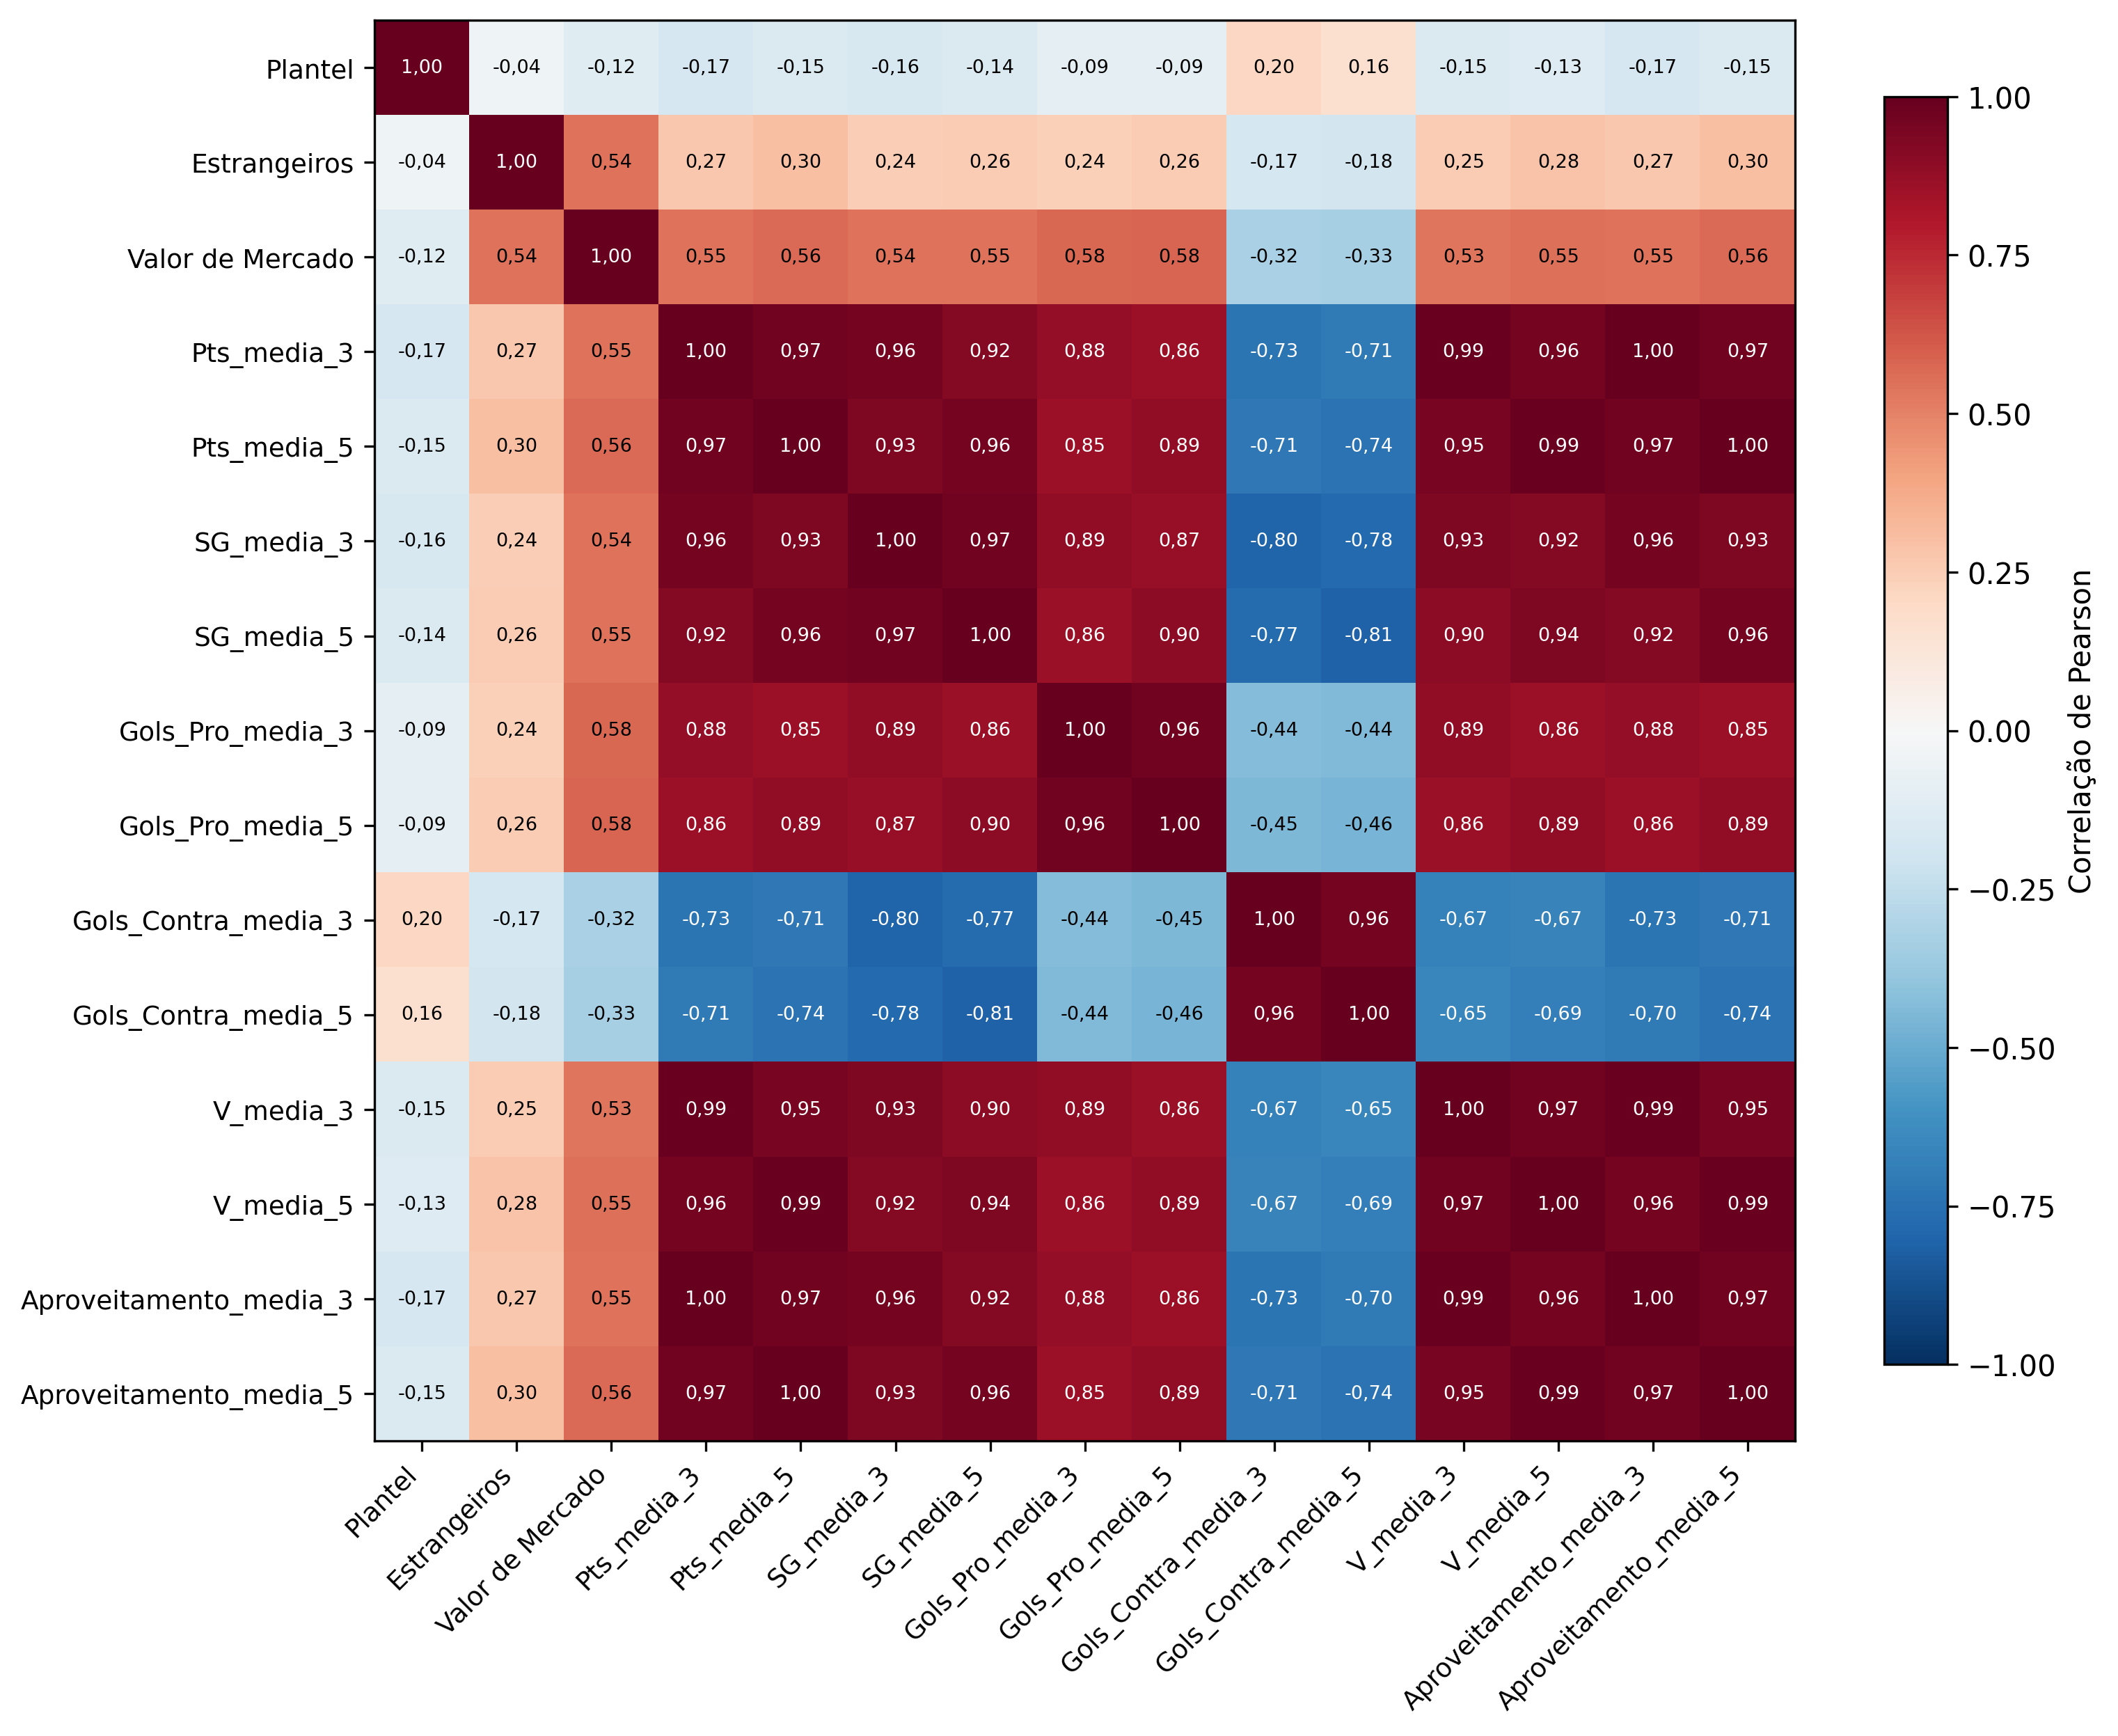
\includegraphics[width=0.95\textwidth]{heatmap_correlacao.png}
    \caption[Matriz de correlação entre as \textit{features}]{Matriz de correlação de Pearson entre as 15 \textit{features} (base rotulada 2014--2024).}
    \label{fig:heatmap}

    \small \textit{Fonte: Elaborado pelo autor (\the\year).}
\end{figure}

\subsection{Pré-processamento e Tratamento de Dados Faltantes}

Clubes recém-promovidos da Série B não possuem histórico completo na Série A, o que gera valores ausentes nas \textit{features} de janela deslizante. Esses valores foram imputados com a \textbf{mediana calculada exclusivamente no conjunto de treinamento}, decisão que se justifica por três razões: (i) a mediana é robusta a valores extremos, adequada a distribuições assimétricas como as de desempenho esportivo; (ii) calculá-la apenas no treino evita que estatísticas do conjunto de teste contaminem o ajuste do modelo; e (iii) a imputação por um valor central é conservadora --- atribui ao clube sem histórico um comportamento ``típico'', sem induzir viés otimista ou pessimista. Em seguida, todas as \textit{features} foram padronizadas com \textit{StandardScaler}, com parâmetros ajustados somente no conjunto de treinamento e aplicados aos demais conjuntos, novamente evitando vazamento de dados.

O desbalanceamento de classes ($\sim$20\% de rebaixados) foi tratado no nível dos algoritmos, com ponderação inversa à frequência das classes (\texttt{class\_weight='balanced'} na Regressão Logística, no \textit{Random Forest} e no LightGBM; \texttt{scale\_pos\_weight}=4 no XGBoost).

\subsection{Separação Temporal e Validação \textit{Walk-Forward}}

Os dados rotulados foram divididos temporalmente em treinamento (2014--2022, 180 observações) e teste (2023--2024, 40 observações, sendo 8 rebaixamentos). Sobre o conjunto de treinamento aplicou-se a validação \textit{walk-forward} com cinco partições (\textit{folds}) de janela expansiva, conforme a Tabela~\ref{tab:folds}: em cada \textit{fold}, o modelo é treinado com todas as temporadas até o ano anterior e validado na temporada seguinte, com imputação e padronização recalculadas dentro de cada \textit{fold} para preservar a integridade temporal.

\begin{table}[htbp]
    \centering
    \caption{Configuração dos cinco \textit{folds} da validação \textit{walk-forward}.}
    \label{tab:folds}
    \begin{tabular}{cccc}
        \toprule
        \textbf{\textit{Fold}} & \textbf{Conjunto de Treino} & \textbf{Validação} & \textbf{Obs. de Treino} \\
        \midrule
        1 & 2014--2017 & 2018 & $\sim$80 \\
        2 & 2014--2018 & 2019 & $\sim$100 \\
        3 & 2014--2019 & 2020 & $\sim$120 \\
        4 & 2014--2020 & 2021 & $\sim$140 \\
        5 & 2014--2021 & 2022 & $\sim$160 \\
        \bottomrule
    \end{tabular}

    \vspace{2pt}
    {\small Fonte: Elaborado pelo autor (\the\year).}
\end{table}


\subsection{Seleção de Algoritmos e Otimização de Hiperparâmetros}

Foram selecionados quatro algoritmos que cobrem o espectro de complexidade usual em dados tabulares: a Regressão Logística, como modelo linear interpretável de referência; o \textit{Random Forest}, como \textit{ensemble} de \textit{bagging}; e XGBoost e LightGBM, como representantes do estado da arte em \textit{gradient boosting} para dados tabulares \cite{chen2016, ke2017}. Redes neurais profundas foram deliberadamente excluídas: com apenas $\sim$220 observações, modelos com grande número de parâmetros tendem ao sobreajuste e não dispõem de volume de dados suficiente para exibir suas vantagens \cite{geron2022}.

A otimização de hiperparâmetros utilizou \textit{RandomizedSearchCV} com 30 candidatos por modelo, validação interna \textit{TimeSeriesSplit} de 5 \textit{folds} e AUC-ROC como critério de seleção. A busca aleatória foi preferida à busca em grade (\textit{GridSearchCV}) porque, para um mesmo orçamento computacional, explora o espaço de hiperparâmetros de forma mais eficiente, especialmente quando apenas algumas dimensões são realmente relevantes \cite{bergstra2012}; métodos de otimização bayesiana foram considerados, mas o ganho esperado não justificaria a complexidade adicional para um espaço de busca deste porte.

% ============================================================
% 4. RESULTADOS E DISCUSSÃO
% ============================================================
\section{Resultados e Discussão}

\subsection{Validação \textit{Walk-Forward}}

A Tabela~\ref{tab:walkforward} apresenta o AUC-ROC de cada modelo em cada \textit{fold} da validação \textit{walk-forward}. A Regressão Logística obteve a maior média (0,794) com o menor desvio padrão ($\pm$0,058), evidenciando comportamento estável ao longo das temporadas. O LightGBM, por sua vez, apresentou a maior variância entre \textit{folds} ($\pm$0,151), com desempenho que oscila de 0,438 (temporada 2020, marcada pelas condições atípicas da pandemia) a 0,906 (2022). Essa instabilidade sugere que modelos de \textit{boosting}, mais flexíveis, são também mais sensíveis a mudanças de regime nos dados --- observação que corrobora a recomendação de \citeonline{bergmeir2012} de avaliar preditores temporais em múltiplas janelas de validação, e não em um único corte.

\begin{table}[htbp]
    \centering
    \caption{AUC-ROC por \textit{fold} da validação \textit{walk-forward}.}
    \label{tab:walkforward}
    \begin{tabular}{lcccc}
        \toprule
        \textbf{\textit{Fold} (ano val.)} & \textbf{Reg. Logística} & \textbf{\textit{Random Forest}} & \textbf{XGBoost} & \textbf{LightGBM} \\
        \midrule
        \textit{Fold} 1 --- 2018 & 0,828 & 0,789 & 0,766 & 0,719 \\
        \textit{Fold} 2 --- 2019 & 0,859 & 0,734 & 0,719 & 0,750 \\
        \textit{Fold} 3 --- 2020 & 0,703 & 0,758 & 0,531 & 0,438 \\
        \textit{Fold} 4 --- 2021 & 0,750 & 0,656 & 0,594 & 0,688 \\
        \textit{Fold} 5 --- 2022 & 0,828 & 0,875 & 0,688 & 0,906 \\
        \midrule
        \textbf{Média $\pm$ DP} & \textbf{0,794 $\pm$ 0,058} & 0,762 $\pm$ 0,071 & 0,659 $\pm$ 0,085 & 0,700 $\pm$ 0,151 \\
        \bottomrule
    \end{tabular}

    \vspace{2pt}
    {\small Fonte: Elaborado pelo autor (\the\year).}
\end{table}


O \textit{fold} 3, correspondente à temporada 2020, merece exame específico: foi o pior para todos os modelos, com o LightGBM atingindo AUC-ROC de 0,438 --- abaixo, inclusive, do classificador aleatório --- e o XGBoost, 0,531. A temporada 2020 foi disputada sob os efeitos da pandemia de COVID-19: iniciada apenas em agosto de 2020 e encerrada em fevereiro de 2021, transcorreu com estádios vazios, calendário comprimido, surtos de contágio nos elencos e desgaste físico atípico. Nessas condições, a relação histórica entre as \textit{features} pré-temporada e o desempenho em campo foi parcialmente rompida --- um choque exógeno que modelos alimentados exclusivamente com informações estruturais não têm como antecipar. O episódio evidencia uma limitação inerente à abordagem pré-temporada e, ao mesmo tempo, fortalece a proposta de trabalho futuro de retreinamento parcial ao longo da temporada, capaz de incorporar sinais correntes e reagir a mudanças de regime. Nota-se, por fim, que a Regressão Logística foi o modelo menos afetado no \textit{fold} pandêmico (0,703), comportamento coerente com a menor variância esperada de modelos mais simples.

\subsection{Hiperparâmetros Selecionados}

A Tabela~\ref{tab:hiperparametros} resume as melhores configurações encontradas pela busca aleatória. Nota-se que os \textit{ensembles} convergiram para configurações conservadoras (profundidades reduzidas, taxas de aprendizado baixas), coerentes com o volume modesto de dados --- árvores rasas limitam a capacidade do modelo e mitigam o sobreajuste.

\begin{table}[htbp]
    \centering
    \caption[Hiperparâmetros selecionados]{Hiperparâmetros selecionados por \textit{RandomizedSearchCV} (30 candidatos) com \textit{TimeSeriesSplit} (5 \textit{folds}) e AUC-ROC como critério de seleção.}
    \label{tab:hiperparametros}
    \small
    \begin{tabular}{lp{7.4cm}c}
        \toprule
        \textbf{Modelo} & \textbf{Melhores Hiperparâmetros (CV)} & \textbf{AUC-ROC CV} \\
        \midrule
        Regressão Logística & $C = 0{,}985$; \textit{solver} = lbfgs & 0,754 \\
        \textit{Random Forest} & \textit{n\_estimators} = 100; \textit{max\_depth} = 3; \textit{min\_samples\_split} = 10; \textit{max\_features} = sqrt & 0,760 \\
        XGBoost & \textit{n\_estimators} = 50; \textit{max\_depth} = 5; \textit{learning\_rate} = 0,05; \textit{subsample} = 0,7 & 0,742 \\
        LightGBM & \textit{n\_estimators} = 50; \textit{max\_depth} = 7; \textit{learning\_rate} = 0,01; \textit{num\_leaves} = 31 & 0,721 \\
        \bottomrule
    \end{tabular}

    \vspace{2pt}
    {\small Fonte: Elaborado pelo autor (\the\year).}
\end{table}


\subsection{Avaliação no Conjunto de Teste Independente}

Após a otimização, cada modelo foi reavaliado no conjunto de teste (2023--2024), não utilizado em nenhuma etapa anterior. A Tabela~\ref{tab:resultados} apresenta o ranqueamento por AUC-ROC, e a Figura~\ref{fig:roc} exibe as curvas ROC correspondentes. O LightGBM alcançou o melhor AUC-ROC (0,877), seguido do \textit{Random Forest} (0,844) e da Regressão Logística (0,828); o XGBoost, embora tenha registrado acurácia idêntica à do LightGBM (82,5\%), obteve o menor AUC-ROC (0,652), caso examinado em detalhe na Seção~\ref{sec:armadilha}. A Figura~\ref{fig:metricas} compara visualmente as métricas, e a Figura~\ref{fig:matrizes} apresenta as matrizes de confusão dos quatro modelos.

\begin{table}[htbp]
    \centering
    \caption[Ranqueamento dos modelos no teste]{Ranqueamento dos modelos por AUC-ROC no conjunto de teste independente (2023--2024).}
    \label{tab:resultados}
    \begin{tabular}{clcc}
        \toprule
        \textbf{Rank} & \textbf{Modelo} & \textbf{AUC-ROC} & \textbf{Acurácia} \\
        \midrule
        1.\textordmasculine{} & LightGBM            & \textbf{0,877} & 82,5\% \\
        2.\textordmasculine{} & \textit{Random Forest} & 0,844 & 80,0\% \\
        3.\textordmasculine{} & Regressão Logística & 0,828 & 80,0\% \\
        4.\textordmasculine{} & XGBoost             & 0,652 & 82,5\% \\
        \bottomrule
    \end{tabular}

    \vspace{2pt}
    {\small Fonte: Elaborado pelo autor (\the\year).}
\end{table}


\begin{figure}[htbp]
    \centering
    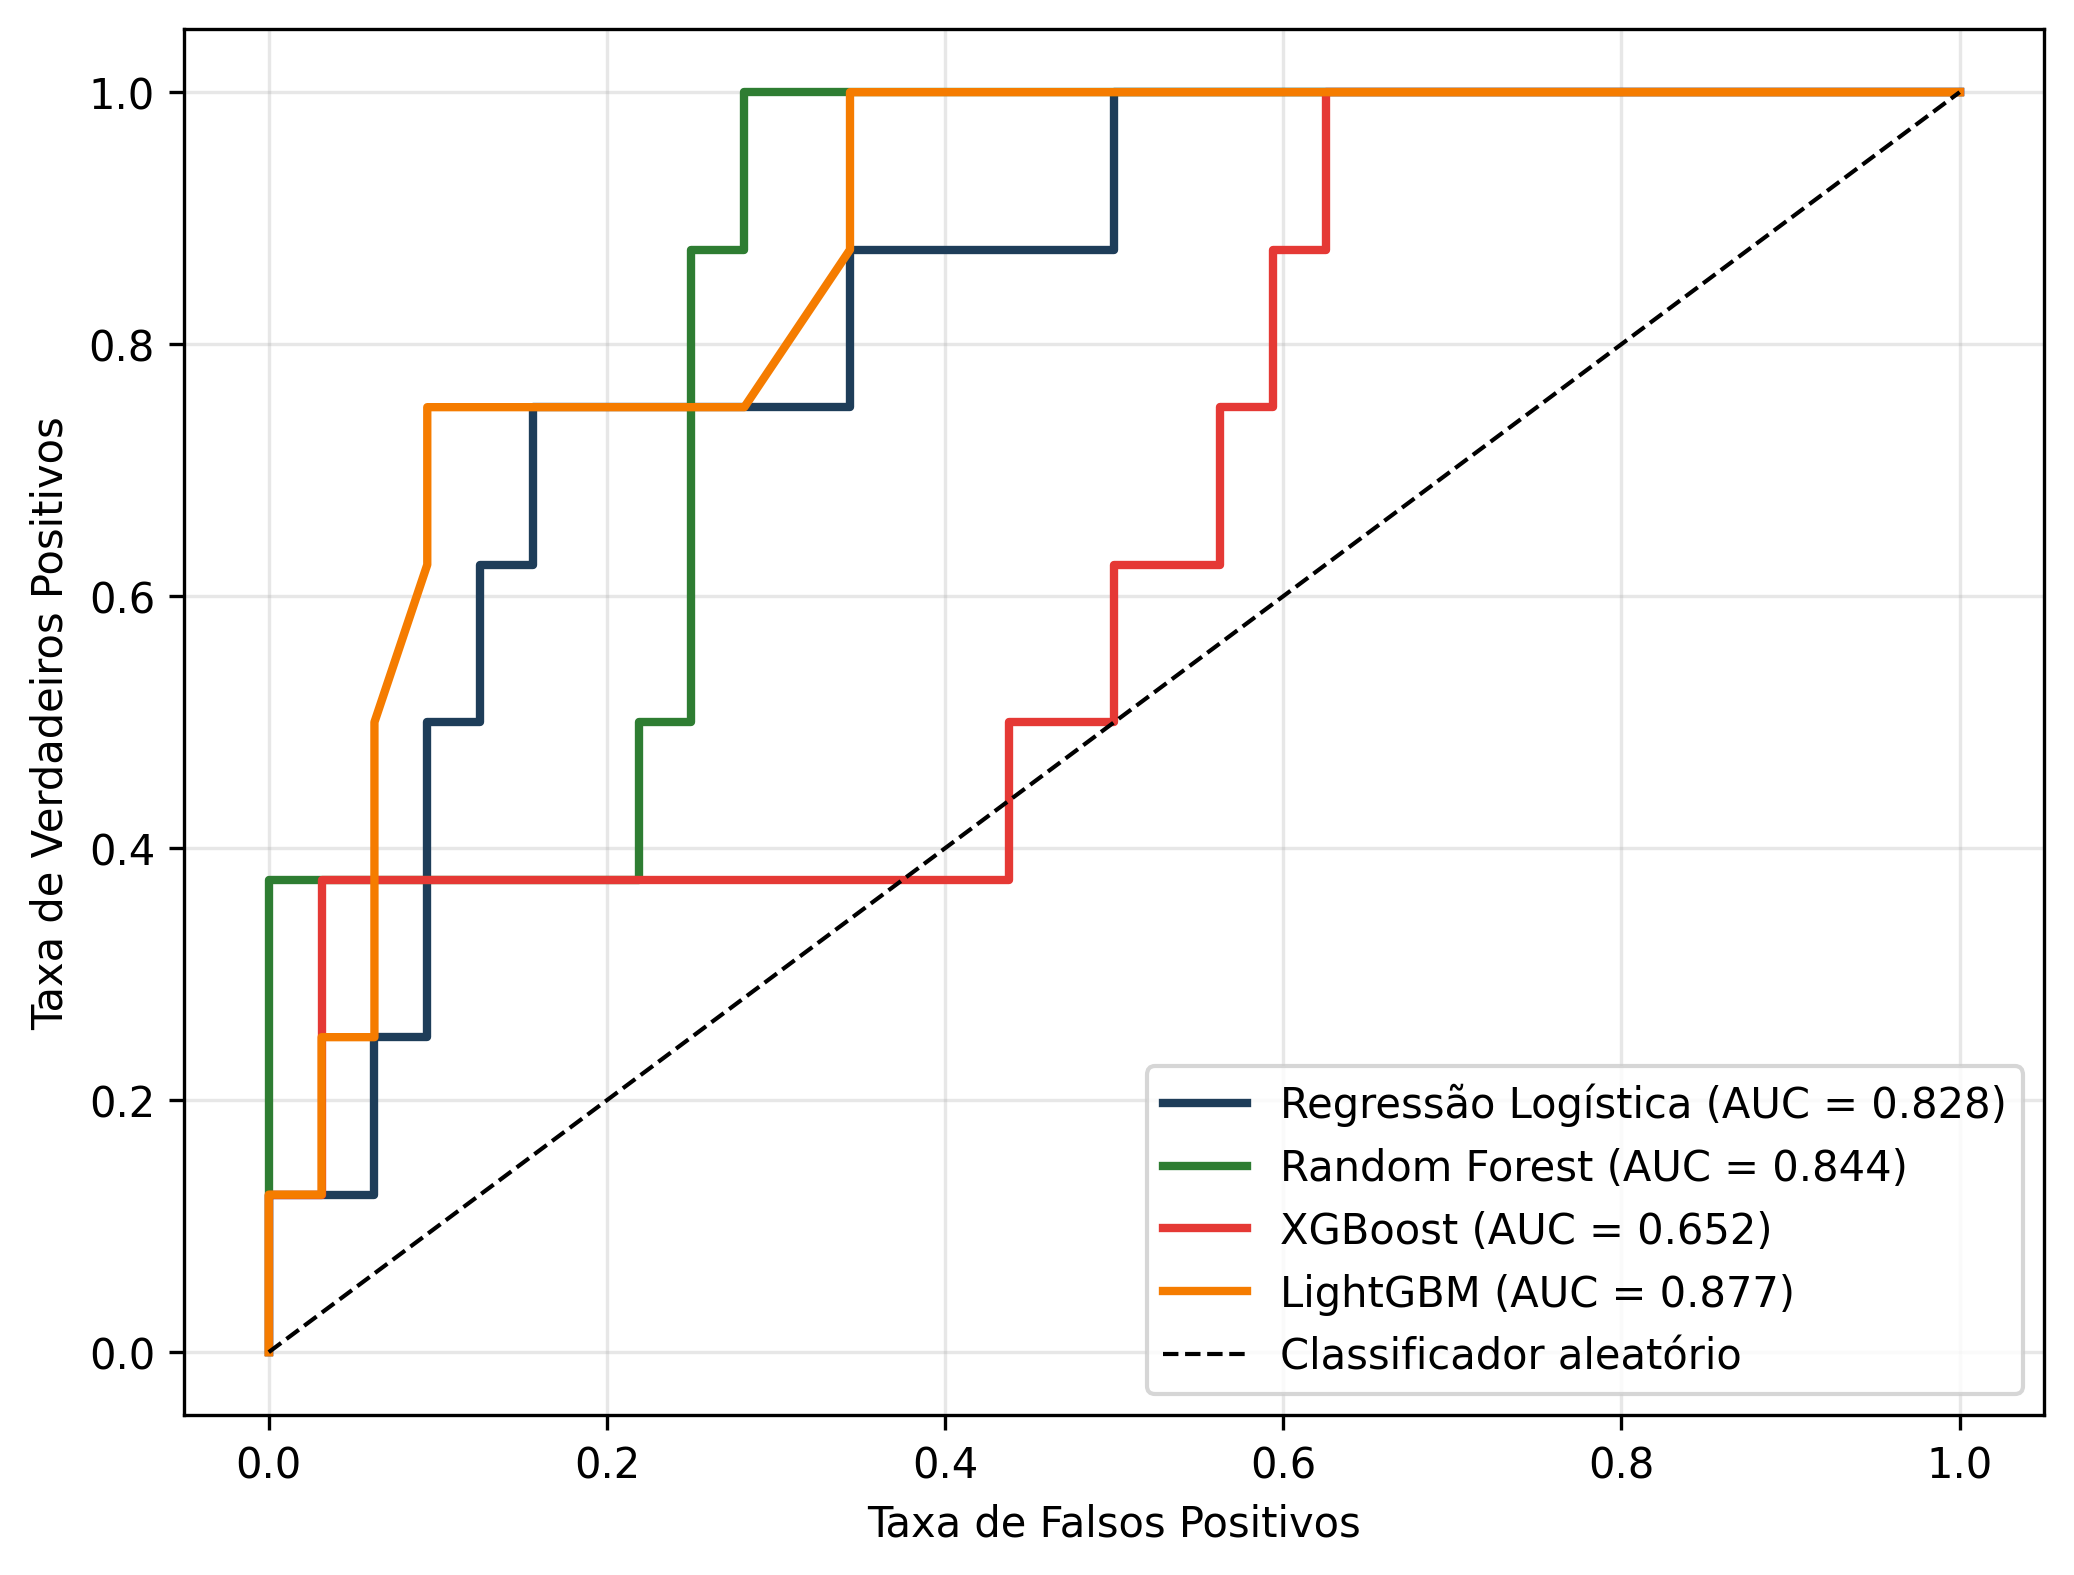
\includegraphics[width=0.75\textwidth]{roc_comparacao_4modelos.png}
    \caption[Curvas ROC dos quatro modelos no teste]{Curvas ROC dos quatro modelos no conjunto de teste (2023--2024). A diagonal tracejada representa um classificador aleatório (AUC = 0,50).}
    \label{fig:roc}

    \small \textit{Fonte: Elaborado pelo autor (\the\year).}
\end{figure}

\begin{figure}[htbp]
    \centering
    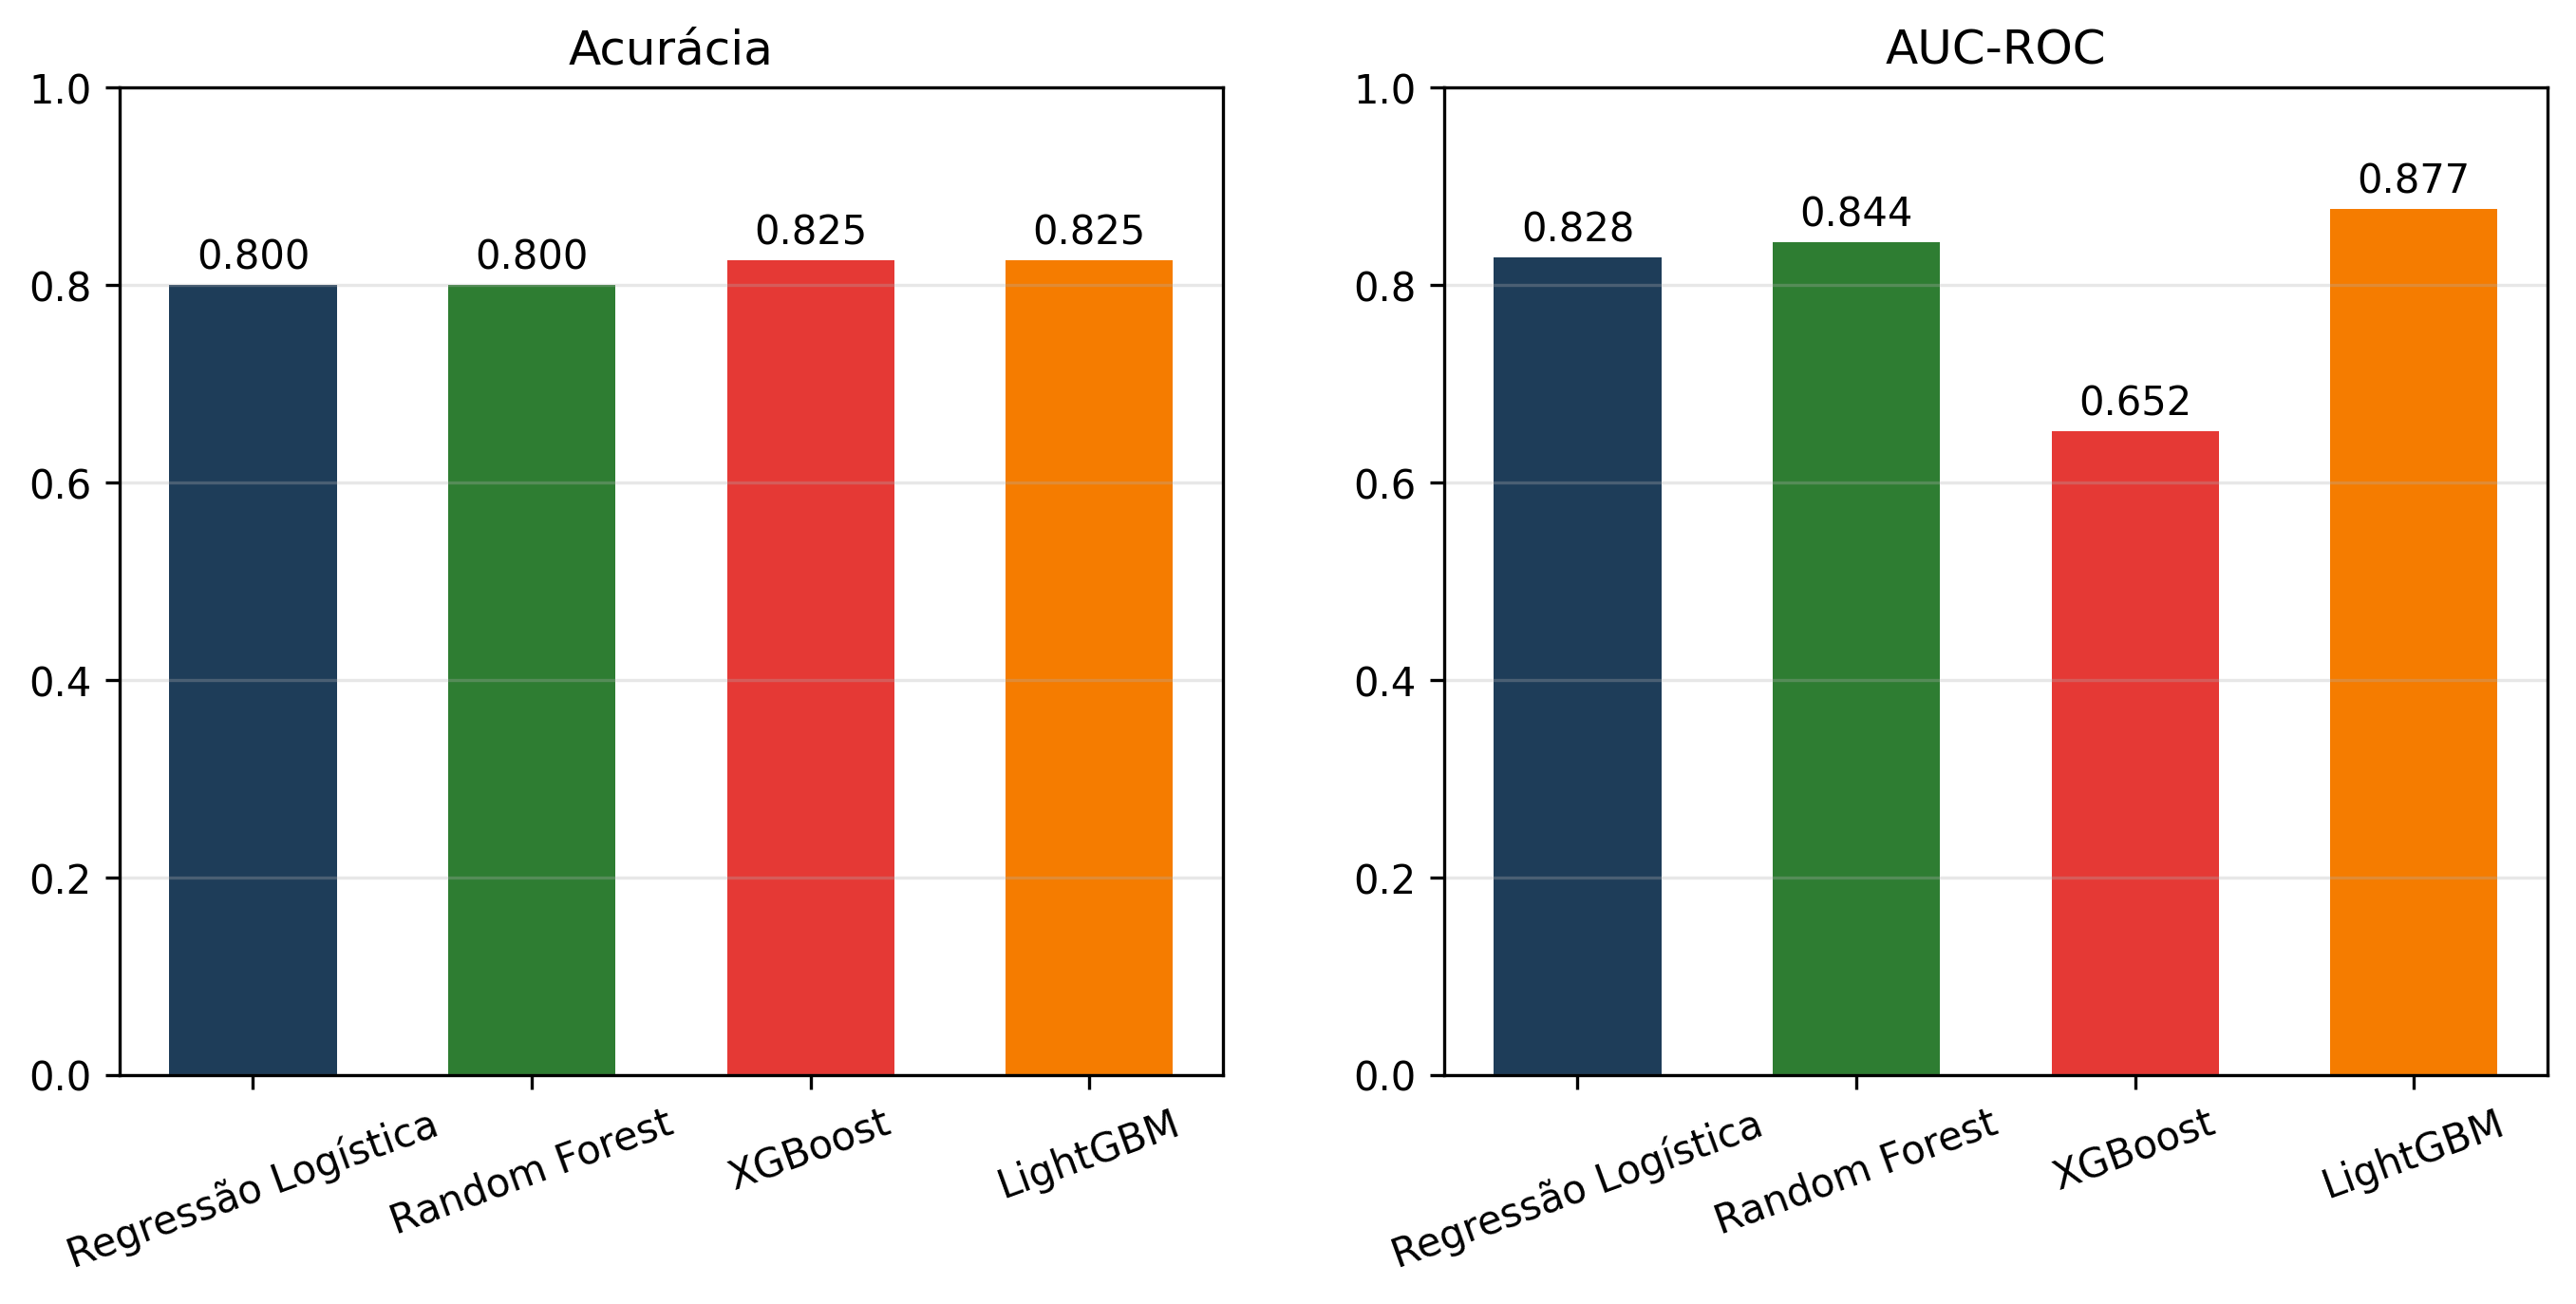
\includegraphics[width=0.95\textwidth]{comparacao_metricas_4modelos.png}
    \caption[Comparação das métricas entre os modelos]{Comparação das métricas de desempenho (Acurácia e AUC-ROC) entre os modelos no conjunto de teste.}
    \label{fig:metricas}

    \small \textit{Fonte: Elaborado pelo autor (\the\year).}
\end{figure}

\begin{figure}[htbp]
    \centering
    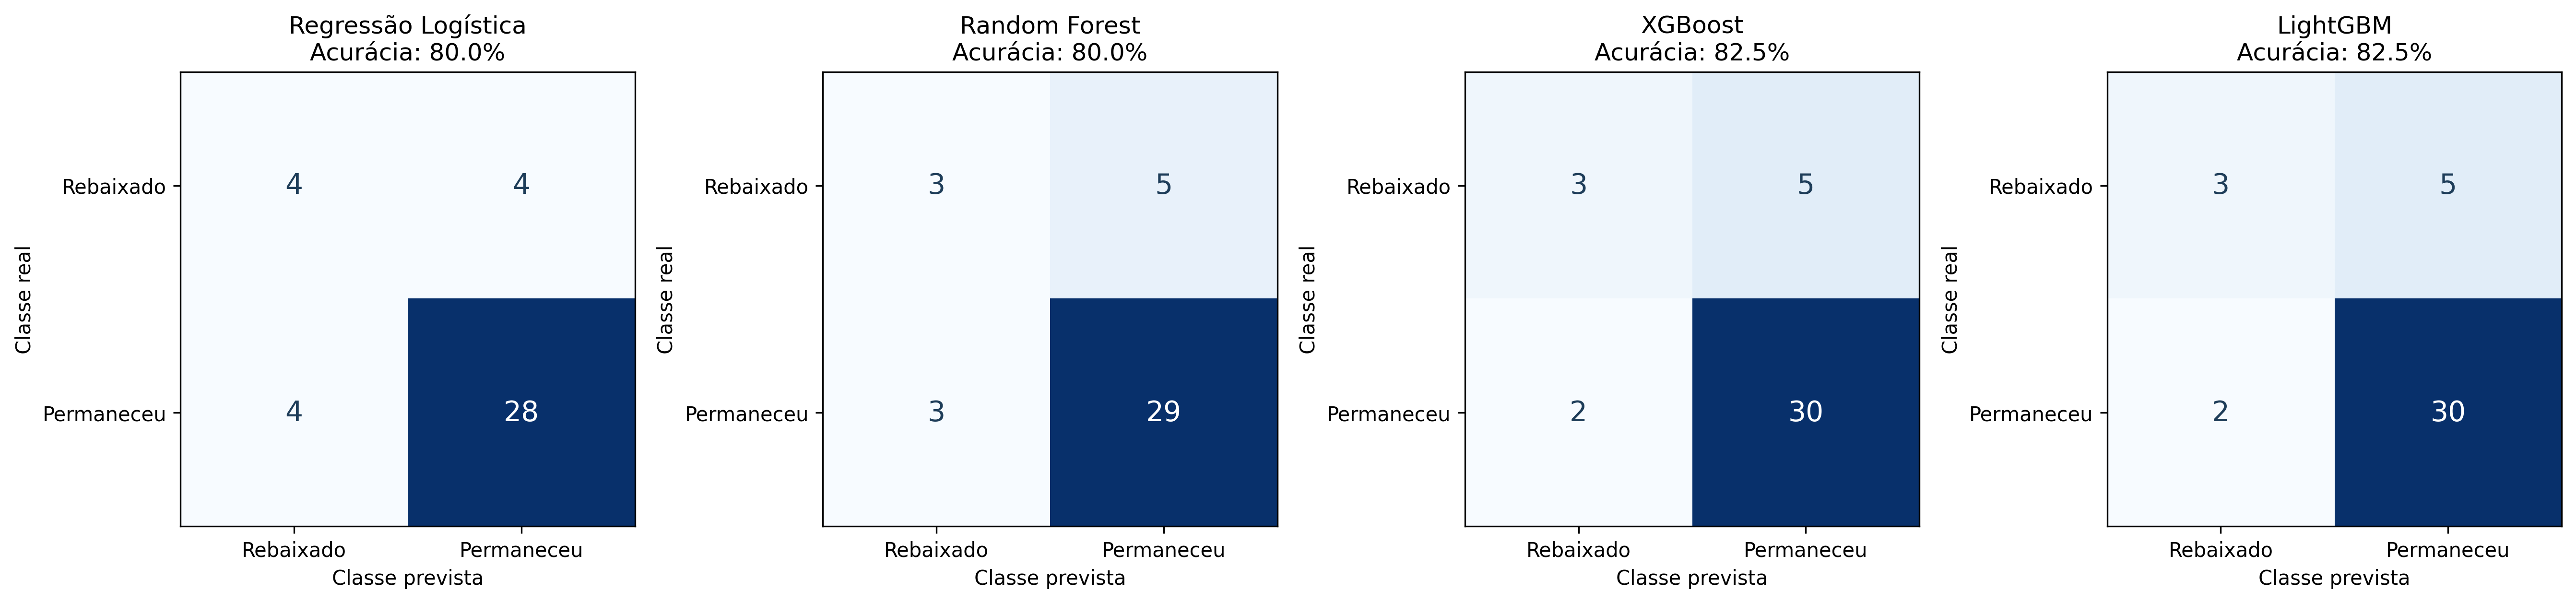
\includegraphics[width=1.0\textwidth]{matrizes_confusao_4modelos.png}
    \caption[Matrizes de confusão dos quatro modelos]{Matrizes de confusão dos quatro modelos no conjunto de teste (2023--2024).}
    \label{fig:matrizes}

    \small \textit{Fonte: Elaborado pelo autor (\the\year).}
\end{figure}

A Tabela~\ref{tab:classificacao} detalha o relatório de classificação da Regressão Logística. Observa-se o padrão típico de classes desbalanceadas: desempenho elevado na classe majoritária (F1 = 0,88) e moderado na classe minoritária (F1 = 0,50), reforçando que o valor do modelo está na \emph{ordenação} dos clubes por risco --- capturada pelo AUC-ROC --- mais do que na classificação binária com limiar fixo.

\begin{table}[htbp]
    \centering
    \caption[Relatório de classificação da Regressão Logística]{Relatório de classificação da Regressão Logística no conjunto de teste (2023--2024).}
    \label{tab:classificacao}
    \begin{tabular}{lcccc}
        \toprule
        \textbf{Classe} & \textbf{Precisão} & \textbf{\textit{Recall}} & \textbf{F1-\textit{Score}} & \textbf{Suporte} \\
        \midrule
        Permanece (0)  & 0,88 & 0,88 & 0,88 & 32 \\
        Rebaixado (1)  & 0,50 & 0,50 & 0,50 & 8  \\
        \midrule
        Acurácia geral & ---  & ---  & 0,80 & 40 \\
        Média macro    & 0,69 & 0,69 & 0,69 & 40 \\
        Média ponderada & 0,80 & 0,80 & 0,80 & 40 \\
        \bottomrule
    \end{tabular}

    \vspace{2pt}
    {\small Fonte: Elaborado pelo autor (\the\year).}
\end{table}


Complementarmente, avaliou-se a calibração das probabilidades da Regressão Logística no conjunto de teste (Figura~\ref{fig:calibracao}). Agrupando as previsões em quartis, a fração observada de rebaixamentos acompanha de perto a probabilidade média prevista em cada grupo (no quartil de maior risco, por exemplo, previsão média de 63,6\% contra 50,0\% de rebaixamentos observados), indicando probabilidades razoavelmente bem calibradas --- sem o excesso de confiança que modelos mais flexíveis costumam exibir em amostras pequenas. Essa propriedade é relevante para o uso gerencial do modelo, pois permite interpretar as probabilidades previstas como estimativas honestas de risco, e não apenas como escores de ordenação.

\begin{figure}[htbp]
    \centering
    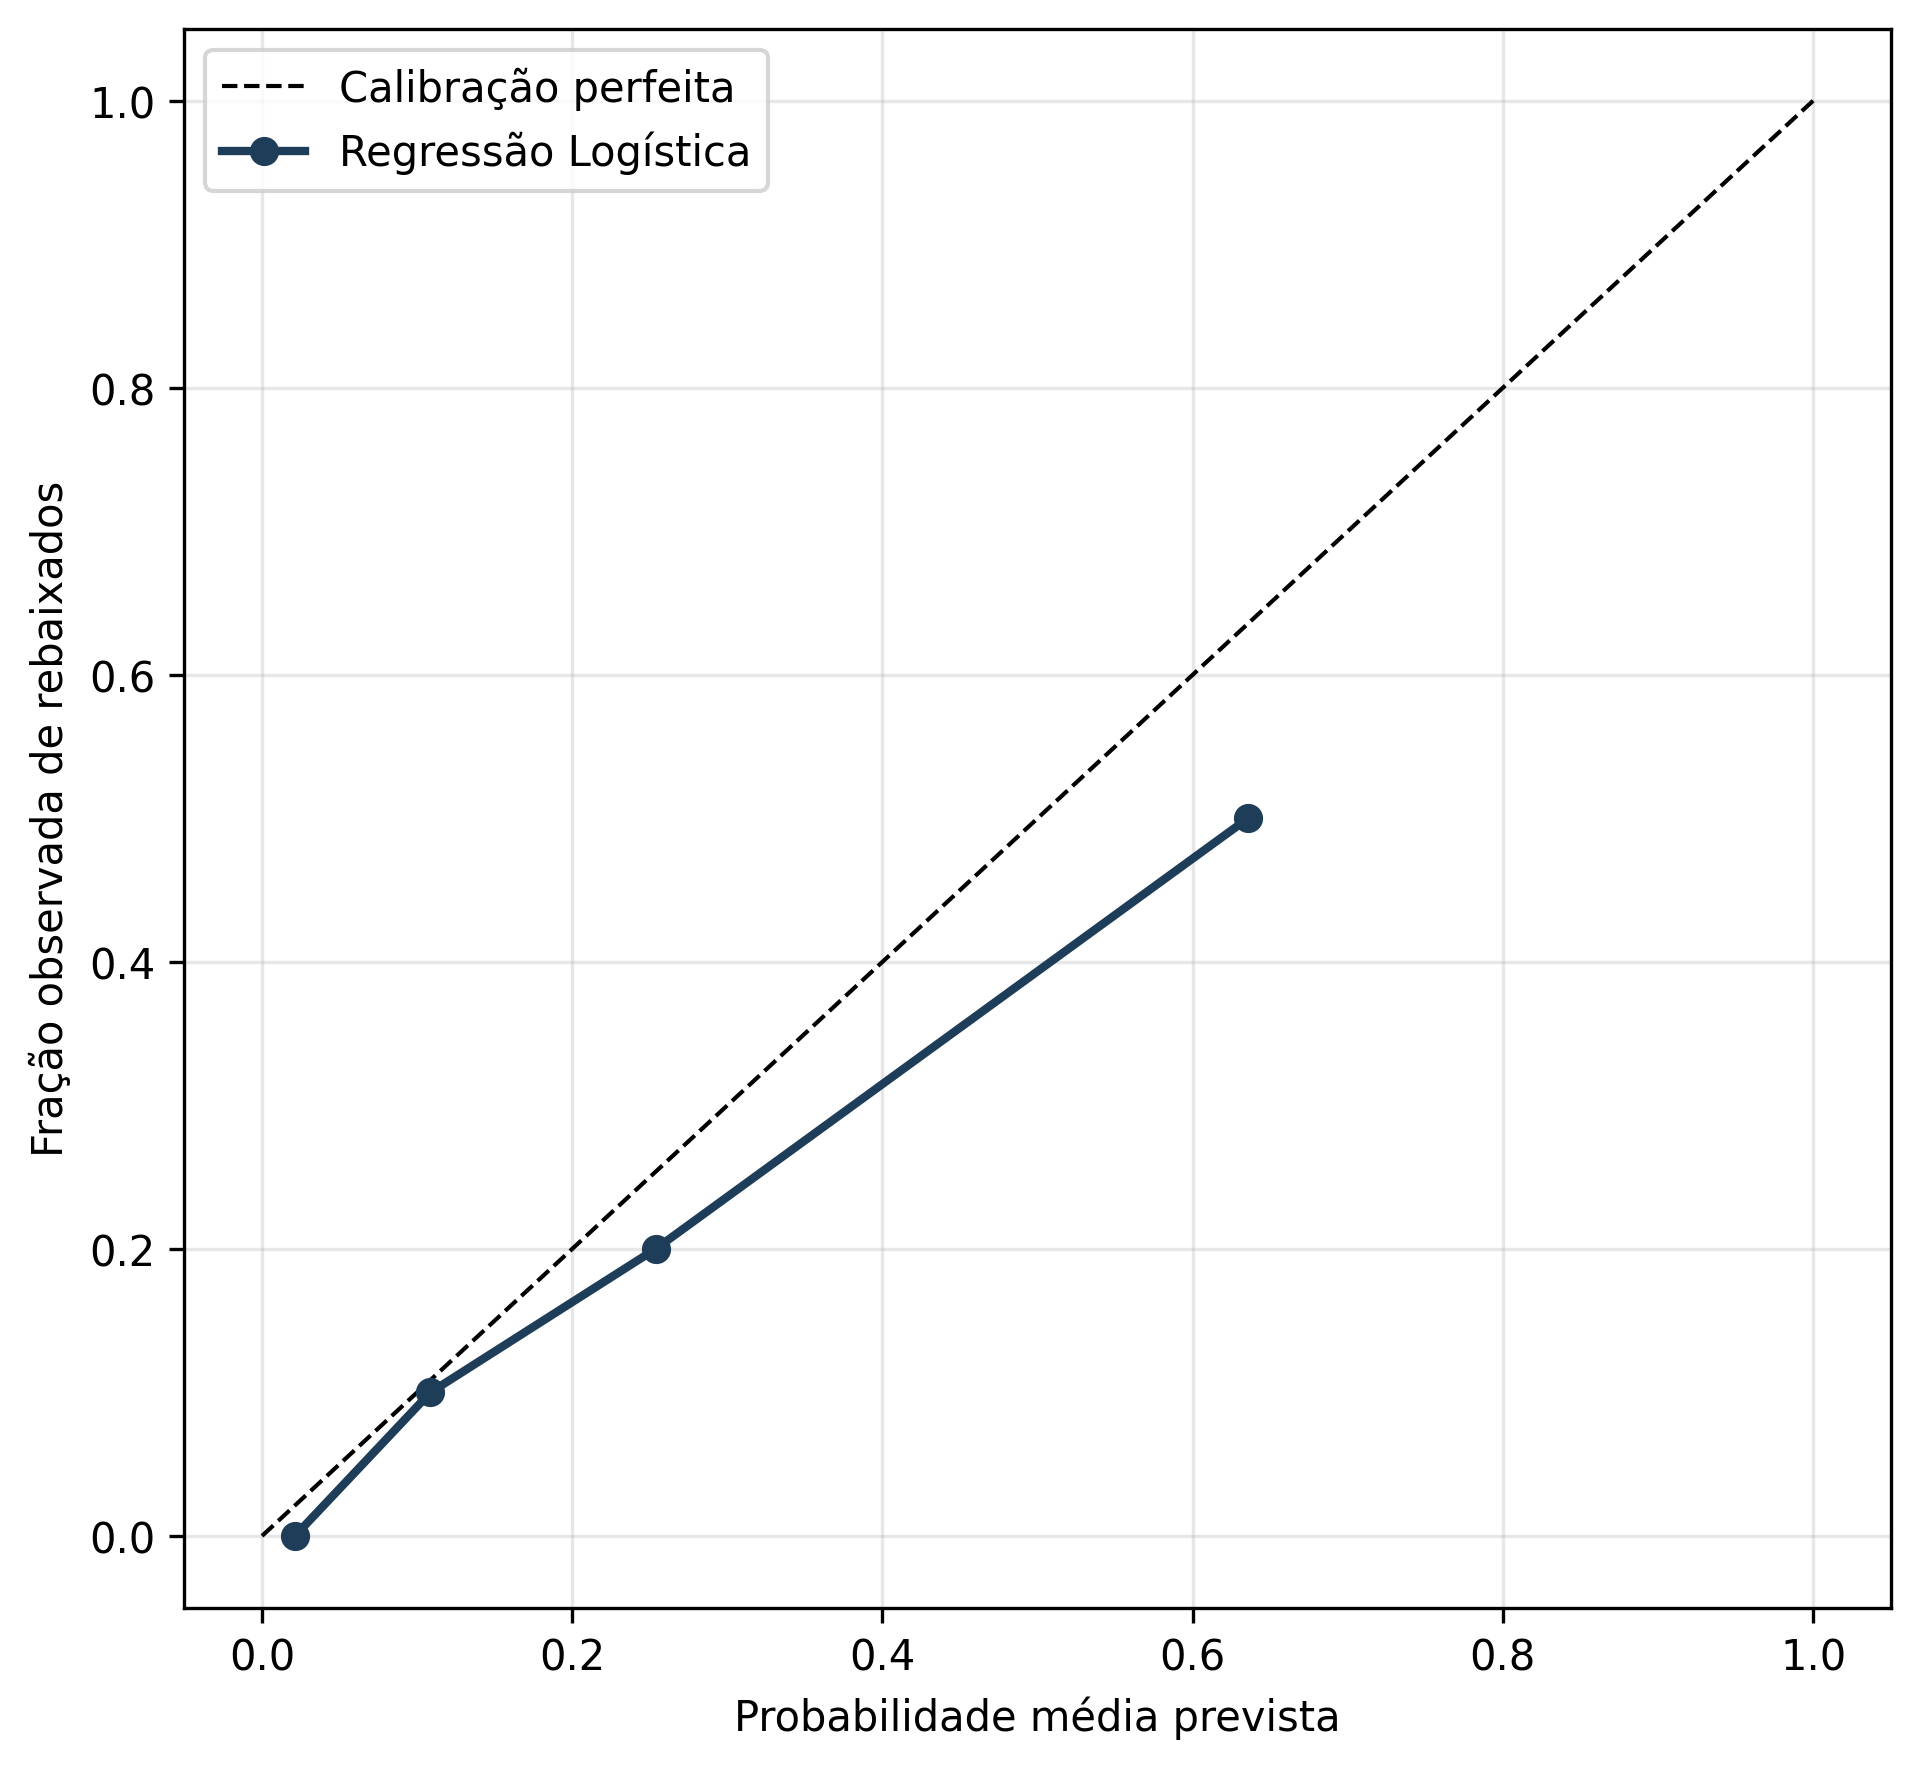
\includegraphics[width=0.6\textwidth]{calibracao_logistica.png}
    \caption[Curva de calibração da Regressão Logística]{Diagrama de confiabilidade (curva de calibração) da Regressão Logística no conjunto de teste (2023--2024), com agrupamento em quartis.}
    \label{fig:calibracao}

    \small \textit{Fonte: Elaborado pelo autor (\the\year).}
\end{figure}

\subsection{Importância das \textit{Features}}
\label{sec:importancia}

A Figura~\ref{fig:importancia} apresenta a importância relativa das \textit{features} sob duas óticas complementares: os coeficientes padronizados da Regressão Logística, cujo sinal indica a direção do efeito sobre o risco, e a importância por ganho do LightGBM, que mede a contribuição de cada variável para as divisões das árvores. Os dois modelos convergem no essencial: o \textbf{valor de mercado do elenco é a variável mais influente em ambos} --- coeficiente de $-0{,}931$ na Regressão Logística (quanto maior o valor, menor o risco previsto) e ganho cerca de quatro vezes superior ao da segunda colocada no LightGBM ---, corroborando \citeonline{muller2017} quanto ao poder preditivo dessa medida. Entre as \textit{features} de desempenho, a média de vitórias nas três temporadas anteriores destaca-se como fator de proteção ($-0{,}703$), confirmando que o histórico recente em campo agrega informação além da dimensão financeira. Chama atenção, ainda, o coeficiente positivo do tamanho do plantel ($+0{,}549$): controlados os demais fatores, elencos mais numerosos associam-se a maior risco --- resultado compatível com a hipótese de que plantéis inchados refletem menor qualidade média por atleta ou instabilidade de planejamento.

Dois cuidados de leitura se impõem, à luz da multicolinearidade diagnosticada na análise exploratória (Figura~\ref{fig:heatmap}). Primeiro, coeficientes de \textit{features} altamente correlacionadas devem ser interpretados em conjunto: os sinais aparentemente contraditórios entre janelas de uma mesma métrica (por exemplo, médias de pontos com coeficiente positivo e médias de vitórias com coeficiente negativo) decorrem da partição de efeito entre variáveis quase colineares, e não de relações causais opostas. Segundo, a concentração do ganho do LightGBM em poucas variáveis sugere redundância entre as janelas de 3 e de 5 temporadas --- uma versão futura do modelo poderia ser simplificada com pouca perda de desempenho.

\begin{figure}[htbp]
    \centering
    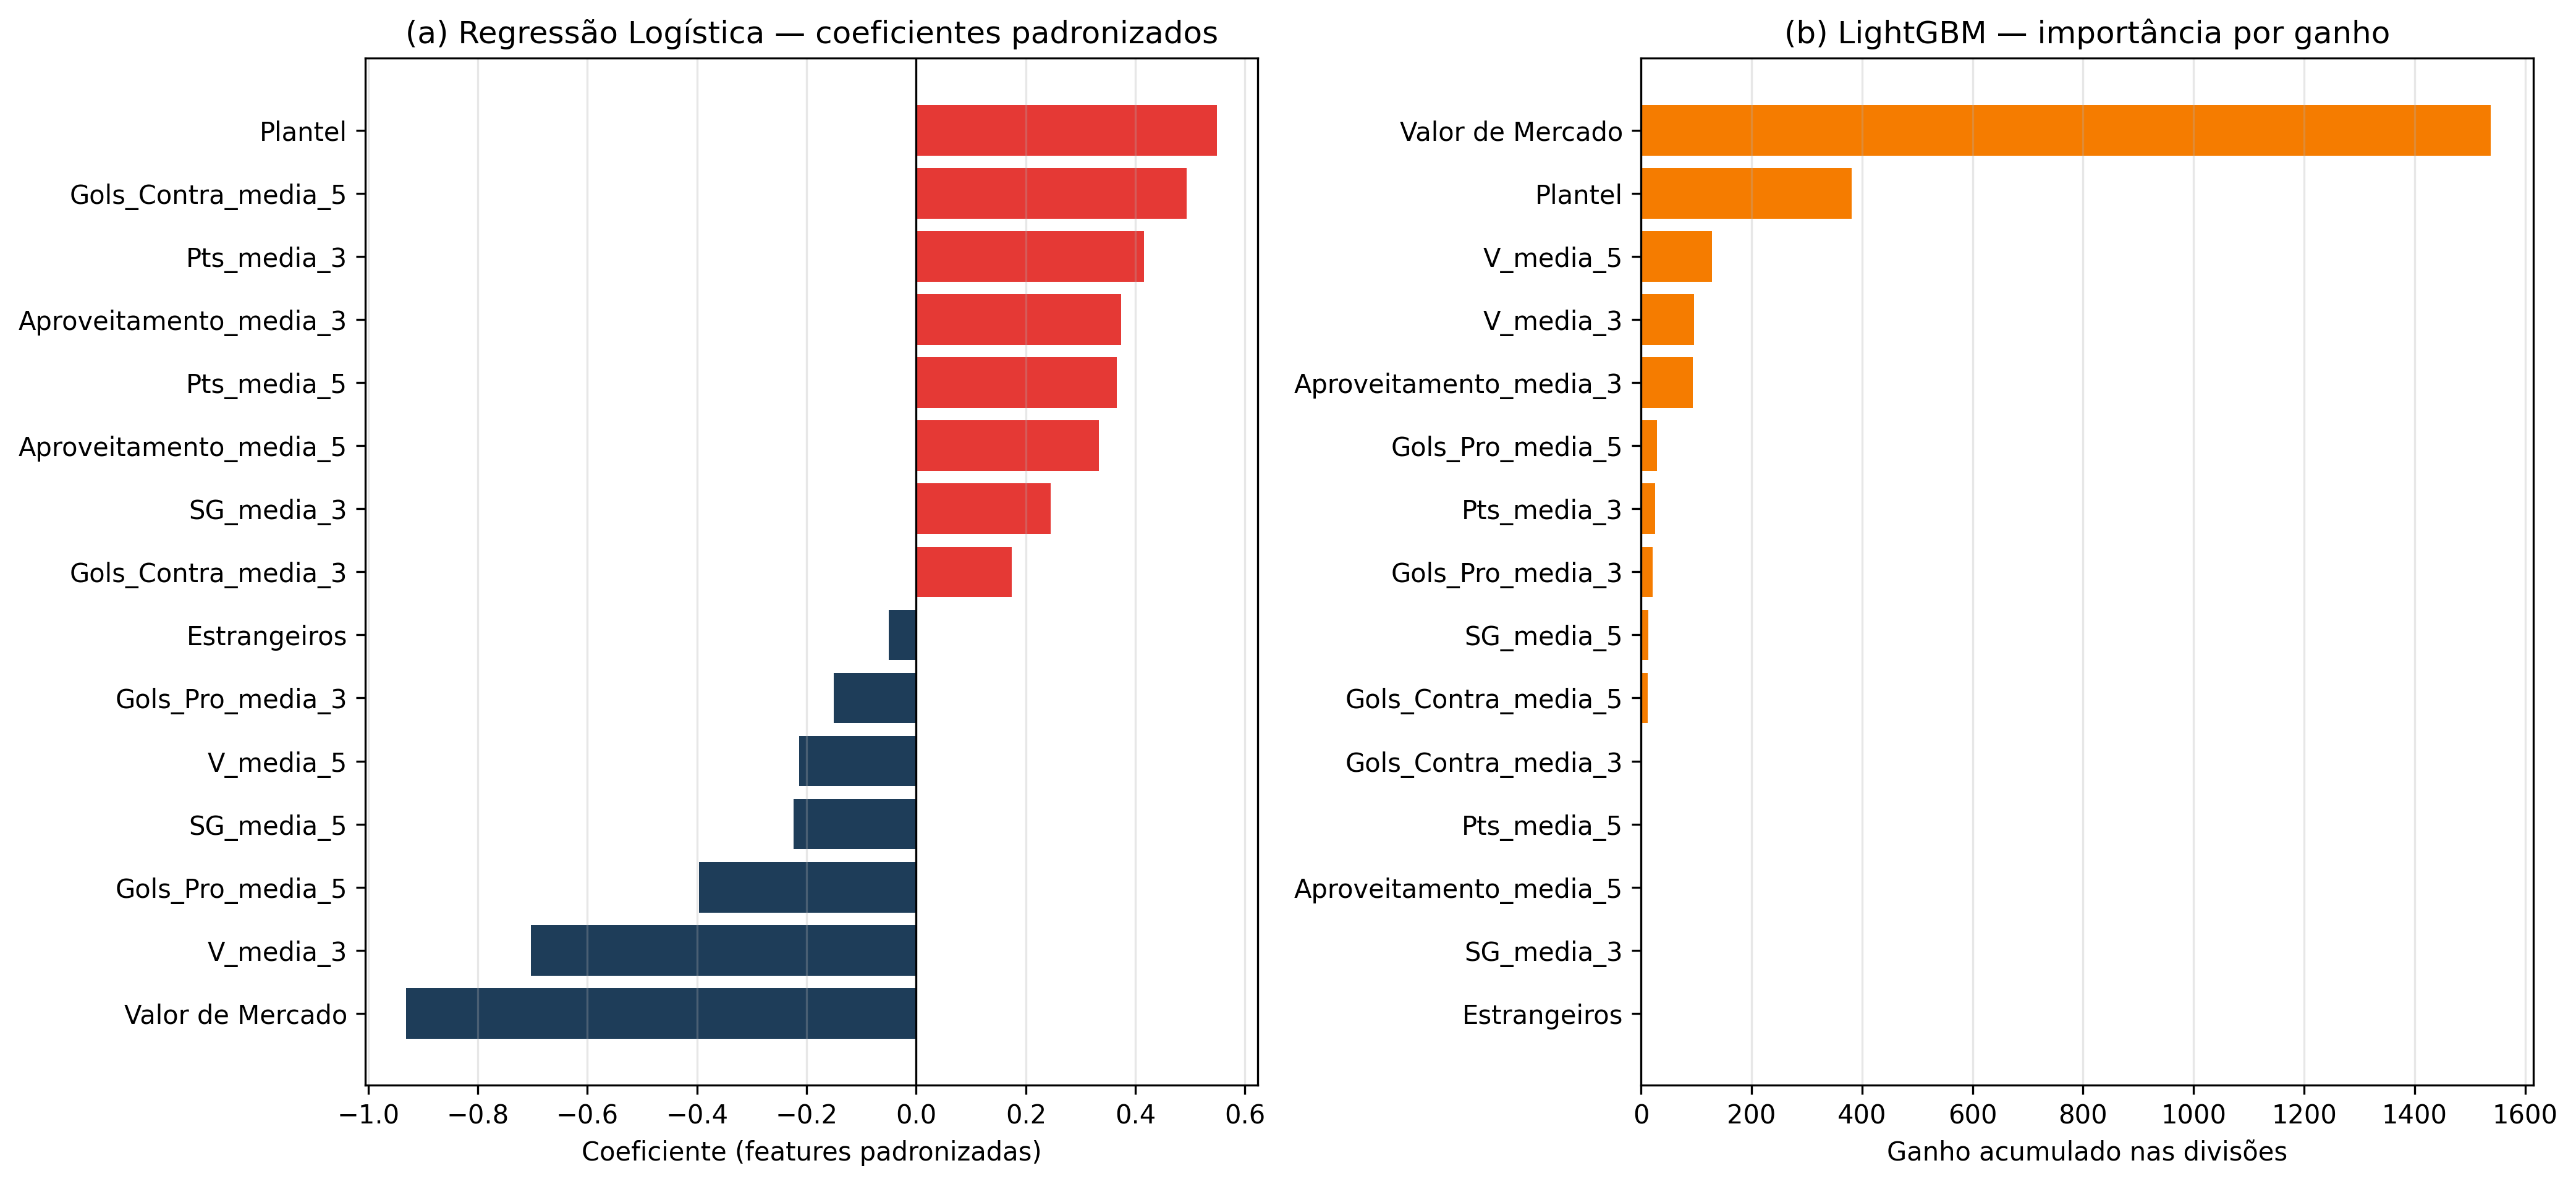
\includegraphics[width=1.0\textwidth]{importancia_features.png}
    \caption[Importância das \textit{features} (RL e LightGBM)]{Importância das \textit{features}: (a) coeficientes padronizados da Regressão Logística final; (b) importância por ganho do LightGBM otimizado.}
    \label{fig:importancia}

    \small \textit{Fonte: Elaborado pelo autor (\the\year).}
\end{figure}

\subsection{A Armadilha da Acurácia: o Caso do XGBoost}
\label{sec:armadilha}

O resultado mais instrutivo da comparação é o contraste do XGBoost: 82,5\% de acurácia --- igual à do LightGBM --- mas AUC-ROC de apenas 0,652. A comparação das matrizes de confusão (Figura~\ref{fig:matrizes}) torna o caso ainda mais eloquente do que a mera igualdade de acurácia sugere: \textbf{as matrizes dos dois modelos são idênticas}. Ambos identificam 3 dos 8 rebaixamentos, incorrem em 5 falsos negativos e 2 falsos positivos e acertam 30 permanências. No limiar de 0,5, portanto, os dois modelos tomam exatamente as mesmas decisões --- e ambos exibem o viés para a classe majoritária descrito por \citeonline{he2009}, prevendo permanência para 35 dos 40 clubes.

Se as decisões binárias são as mesmas, a diferença de 0,225 no AUC-ROC não pode estar nelas: ela reside inteiramente na \textbf{ordenação das probabilidades}. Ordenando as 40 observações do teste por risco previsto, o LightGBM posiciona os oito clubes efetivamente rebaixados nos lugares 1, 3, 5, 6, 7, 9, 17 e 19; o XGBoost, nos lugares 1, 3, 4, 18, 21, 24, 26 e 28 --- isto é, atribui a cinco clubes que caíram um risco menor que o de mais de vinte clubes que permaneceram. A acurácia enxerga apenas o acerto no limiar e não distingue as duas situações; o AUC-ROC avalia a ordenação completa e as separa com nitidez.

O caso demonstra empiricamente por que a acurácia não deve ser utilizada como métrica única neste tipo de problema e reforça a escolha do AUC-ROC como critério principal deste trabalho. Reforça, ainda, o argumento gerencial desenvolvido na Seção~\ref{sec:tradeoff}: o que interessa ao gestor não é um rótulo binário, mas a lista ordenada dos clubes que merecem atenção --- exatamente aquilo que a acurácia é incapaz de aferir.

\subsection{Estabilidade \textit{versus} Desempenho: Escolha do Modelo Final}
\label{sec:tradeoff}

Os resultados colocam em evidência um compromisso (\textit{trade-off}) clássico. O LightGBM maximiza o AUC-ROC no teste (0,877), mas sua alta variância no \textit{walk-forward} ($\pm$0,151) indica menor consistência entre temporadas. A Regressão Logística, embora terceira no teste (0,828), foi a mais estável na validação temporal ($\pm$0,058) e oferece coeficientes diretamente interpretáveis --- \textit{features} com coeficiente positivo aumentam o risco previsto de rebaixamento, informação diretamente utilizável pela gestão esportiva. Assim, para aplicação prática, a Regressão Logística foi adotada como modelo final de previsão, pela combinação de estabilidade e interpretabilidade; o LightGBM permanece como alternativa quando a maximização do AUC-ROC for o critério prioritário --- escolha que a validação retroativa da temporada 2025 (Seção~\ref{sec:validacao2025}) viria a corroborar.

\subsection{Previsão para a Temporada 2025}

Aplicando o modelo final --- a Regressão Logística, treinada com todo o período 2014--2024 ---, aos 20 clubes participantes da Série A de 2025, obtém-se o ranking de risco da Tabela~\ref{tab:previsao2025}, ilustrado na Figura~\ref{fig:previsao}. Registre-se, para eliminar qualquer ambiguidade, que todas as probabilidades da Tabela~\ref{tab:previsao2025} foram geradas exclusivamente pela Regressão Logística; as previsões correspondentes do LightGBM são apresentadas na Seção~\ref{sec:validacao2025}, no contexto da validação retroativa. Seguindo o formato do campeonato, os quatro clubes de maior probabilidade são classificados na zona de rebaixamento; destaca-se que apenas Juventude, Sport Recife e Vitória superaram o limiar de 50\%, tendo o Mirassol sido incluído pela posição no ranking (4.\textordmasculine{} maior risco).

\begin{table}[htbp]
    \centering
    \caption[Ranking de risco previsto para 2025]{Ranking de risco de rebaixamento para a temporada 2025 (Regressão Logística treinada em 2014--2024). Os quatro primeiros são classificados na zona de rebaixamento.}
    \label{tab:previsao2025}
    \small
    \begin{tabular}{clccc}
        \toprule
        \textbf{\#} & \textbf{Clube} & \textbf{Prob. Rebaixamento} & \textbf{Prob. Permanência} & \textbf{Previsão} \\
        \midrule
        1  & Juventude        & 79,4\% & 20,6\%  & Rebaixado \\
        2  & Sport Recife     & 76,9\% & 23,1\%  & Rebaixado \\
        3  & Vitória          & 76,7\% & 23,3\%  & Rebaixado \\
        4  & Mirassol         & 43,6\% & 56,4\%  & Rebaixado \\
        \midrule
        5  & Ceará            & 35,3\% & 64,7\%  & Permanece \\
        6  & Bahia            & 33,1\% & 66,9\%  & Permanece \\
        7  & Fortaleza        & 27,9\% & 72,1\%  & Permanece \\
        8  & Fluminense       & 25,8\% & 74,2\%  & Permanece \\
        9  & Vasco da Gama    & 24,1\% & 75,9\%  & Permanece \\
        10 & Bragantino       & 13,1\% & 86,9\%  & Permanece \\
        11 & Atlético Mineiro & 9,3\%  & 90,7\%  & Permanece \\
        12 & Internacional    & 9,1\%  & 90,9\%  & Permanece \\
        13 & São Paulo        & 9,0\%  & 91,0\%  & Permanece \\
        14 & Corinthians      & 6,4\%  & 93,6\%  & Permanece \\
        15 & Grêmio           & 5,0\%  & 95,0\%  & Permanece \\
        16 & Cruzeiro         & 4,1\%  & 95,9\%  & Permanece \\
        17 & Santos           & 2,9\%  & 97,1\%  & Permanece \\
        18 & Botafogo         & 2,5\%  & 97,5\%  & Permanece \\
        19 & Flamengo         & 0,2\%  & 99,8\%  & Permanece \\
        20 & Palmeiras        & 0,0\%  & 100,0\% & Permanece \\
        \bottomrule
    \end{tabular}

    \vspace{2pt}
    {\small Fonte: Elaborado pelo autor (\the\year).}
\end{table}


\begin{figure}[htbp]
    \centering
    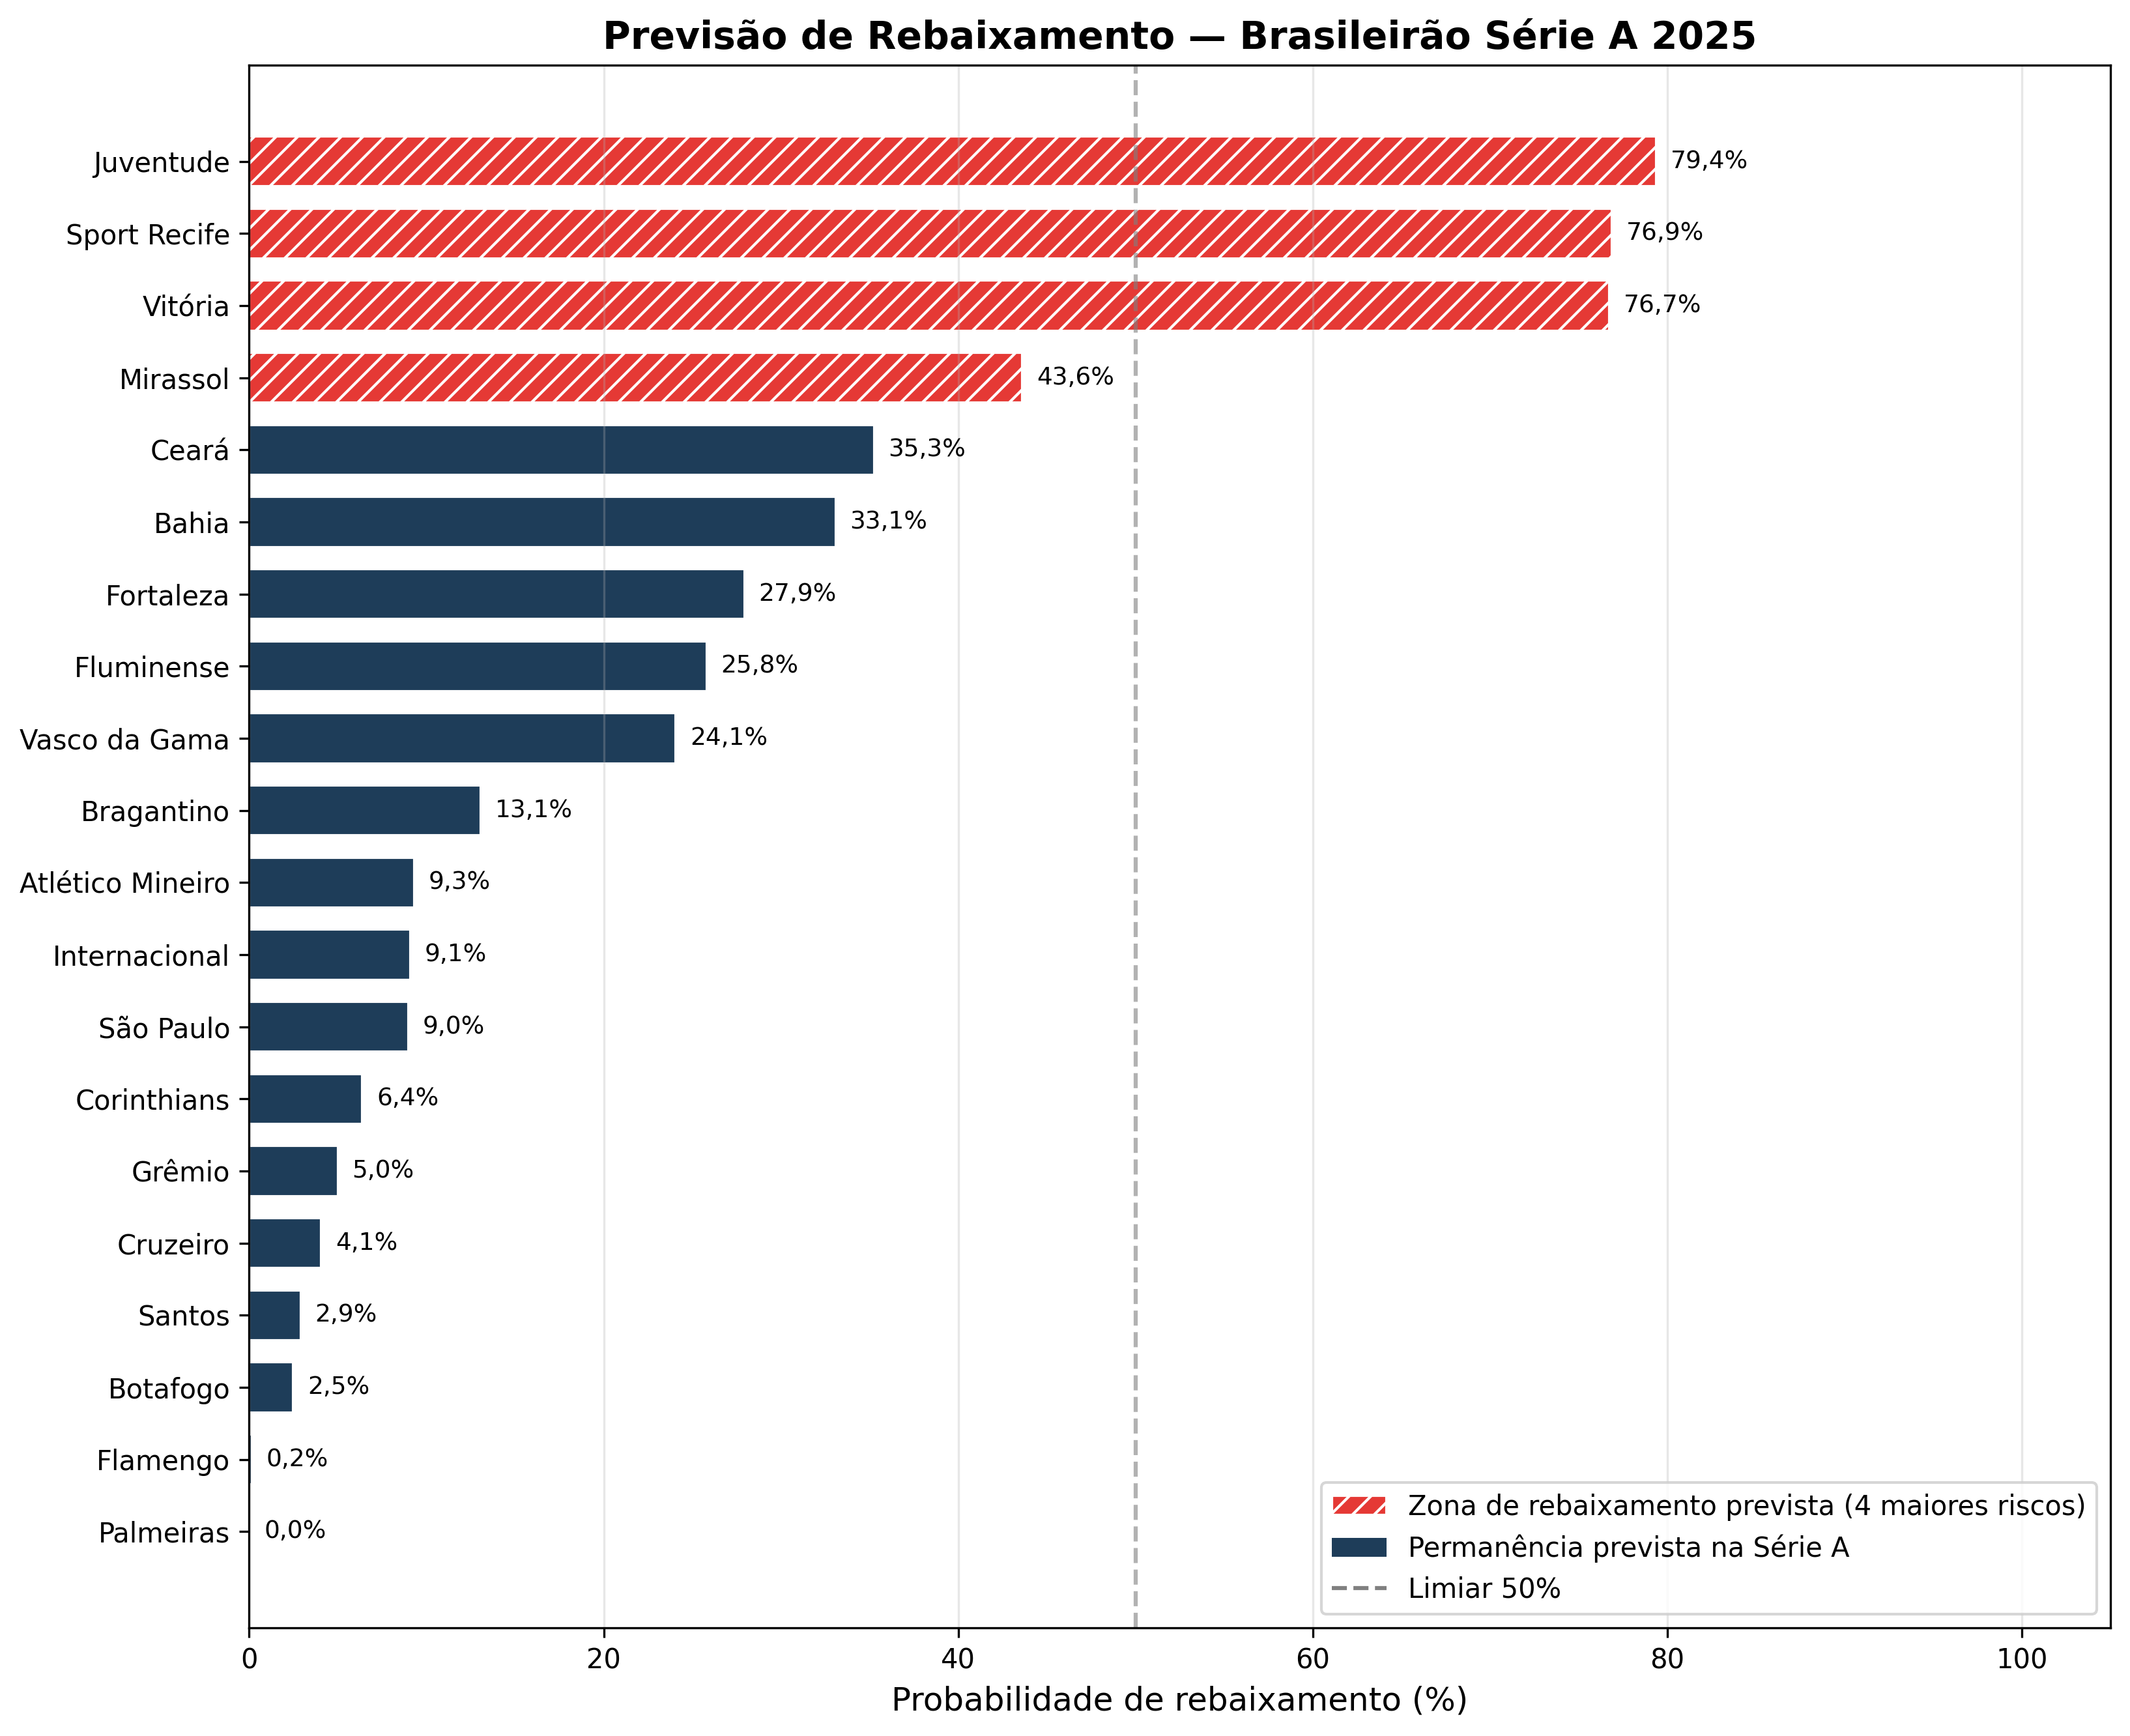
\includegraphics[width=0.9\textwidth]{previsao_2025_v2.png}
    \caption[Ranking de risco de rebaixamento --- 2025]{Ranking de risco de rebaixamento --- Brasileirão Série A 2025. Barras vermelhas hachuradas indicam os quatro clubes previstos para a zona de rebaixamento.}
    \label{fig:previsao}

    \small \textit{Fonte: Elaborado pelo autor (\the\year).}
\end{figure}

As previsões são coerentes com as características que o modelo penaliza: o Juventude acumula baixo aproveitamento nas temporadas recentes; Sport Recife e Vitória são recém-promovidos com elencos de menor valor de mercado; e o Mirassol faz sua estreia histórica na Série A com o menor valor de elenco entre os 20 participantes (\euro 28,4 milhões), dependendo da imputação por mediana nas \textit{features} de histórico --- o que ilustra tanto o funcionamento quanto os limites do modelo para clubes sem passado na elite.

\subsection{Validação Retroativa com os Resultados Oficiais de 2025}
\label{sec:validacao2025}

O Campeonato Brasileiro de 2025 foi concluído em dezembro de 2025, o que permite confrontar a previsão apresentada na seção anterior com o desfecho real --- transformando-a de exercício prospectivo em resultado verificável. Os quatro clubes efetivamente rebaixados foram Sport Recife (20.\textordmasculine{} colocado), Juventude (19.\textordmasculine{}), Fortaleza (18.\textordmasculine{}) e Ceará (17.\textordmasculine{}). A Tabela~\ref{tab:validacao2025} reapresenta o ranking de risco da Regressão Logística, agora acompanhado de intervalos de confiança de 95\% (obtidos por \textit{bootstrap} com $B = 1000$ reamostragens de todo o \textit{pipeline}, da imputação ao ajuste), das probabilidades previstas pelo LightGBM treinado no mesmo período e da posição final real de cada clube.

\begin{table}[htbp]
    \centering
    \caption[Validação retroativa da previsão 2025]{Validação retroativa da previsão 2025: probabilidades da Regressão Logística (com intervalos de confiança de 95\% via \textit{bootstrap}, $B = 1000$) e do LightGBM \textit{versus} o resultado real do campeonato. Clubes em negrito foram efetivamente rebaixados.}
    \label{tab:validacao2025}
    \small
    \begin{tabular}{clcccc}
        \toprule
        \textbf{\#} & \textbf{Clube} & \textbf{Prob. RL} & \textbf{IC 95\%} & \textbf{Prob. LGBM} & \textbf{Pos. real} \\
        \midrule
        1 & \textbf{Juventude} & 79,4\% & [65,6; 92,4] & 62,4\% & 19.\textordmasculine{} \\
        2 & \textbf{Sport Recife} & 76,9\% & [42,0; 94,1] & 52,8\% & 20.\textordmasculine{} \\
        3 & Vitória & 76,7\% & [53,1; 89,5] & 47,2\% & 15.\textordmasculine{} \\
        4 & Mirassol & 43,6\% & [19,8; 56,9] & 47,9\% & 4.\textordmasculine{} \\
        \midrule
        5 & \textbf{Ceará} & 35,3\% & [22,0; 77,1] & 49,2\% & 17.\textordmasculine{} \\
        6 & Bahia & 33,1\% & [2,8; 66,7] & 47,2\% & 7.\textordmasculine{} \\
        7 & \textbf{Fortaleza} & 27,9\% & [11,3; 69,0] & 29,5\% & 18.\textordmasculine{} \\
        8 & Fluminense & 25,8\% & [7,0; 59,5] & 31,5\% & 5.\textordmasculine{} \\
        9 & Vasco da Gama & 24,1\% & [5,5; 75,7] & 52,8\% & 14.\textordmasculine{} \\
        10 & Bragantino & 13,1\% & [3,6; 42,9] & 52,8\% & 10.\textordmasculine{} \\
        11 & Atlético Mineiro & 9,3\% & [0,2; 42,4] & 35,0\% & 11.\textordmasculine{} \\
        12 & Internacional & 9,1\% & [2,3; 28,8] & 32,7\% & 16.\textordmasculine{} \\
        13 & São Paulo & 9,0\% & [1,9; 38,0] & 29,4\% & 8.\textordmasculine{} \\
        14 & Corinthians & 6,4\% & [1,3; 27,7] & 29,4\% & 13.\textordmasculine{} \\
        15 & Grêmio & 5,0\% & [0,7; 31,1] & 43,5\% & 9.\textordmasculine{} \\
        16 & Cruzeiro & 4,1\% & [0,6; 38,3] & 45,6\% & 3.\textordmasculine{} \\
        17 & Santos & 2,9\% & [0,2; 34,5] & 52,8\% & 12.\textordmasculine{} \\
        18 & Botafogo & 2,5\% & [0,0; 66,5] & 37,8\% & 6.\textordmasculine{} \\
        19 & Flamengo & 0,2\% & [0,0; 6,9] & 37,8\% & 1.\textordmasculine{} \\
        20 & Palmeiras & 0,0\% & [0,0; 2,4] & 36,3\% & 2.\textordmasculine{} \\
        \bottomrule
    \end{tabular}

    \vspace{2pt}
    {\small Fonte: Elaborado pelo autor (\the\year), com resultados oficiais da CBF.}
\end{table}


Dos quatro clubes apontados na zona de rebaixamento, o modelo acertou dois --- Juventude e Sport Recife, justamente o primeiro e o segundo maiores riscos previstos. Mais revelador, porém, é o desempenho de ordenação: o AUC-ROC realizado na temporada 2025 foi de \textbf{0,922}, superior tanto ao obtido no conjunto de teste 2023--2024 (0,828) quanto à média da validação \textit{walk-forward} (0,794). Os quatro rebaixados reais figuravam, todos, entre os sete maiores riscos do ranking: Ceará ocupava a 5.\textordmasculine{} posição (35,3\%) e Fortaleza a 7.\textordmasculine{} (27,9\%), imediatamente fora do corte. Dos 64 pares possíveis entre um clube rebaixado e um não rebaixado, o modelo ordenou corretamente 59.

Os dois erros do \textit{top}-4 são instrutivos. O Vitória (3.\textordmasculine{} maior risco, 76,7\%) salvou-se com 45 pontos, em 15.\textordmasculine{} lugar --- um erro de magnitude moderada, já que o clube de fato flertou com a zona de rebaixamento. Já o Mirassol (4.\textordmasculine{} maior risco, 43,6\%) constitui o maior erro do modelo, e o mais informativo: estreante na Série A, o clube realizou campanha extraordinária e terminou em 4.\textordmasculine{} lugar, com 67 pontos, classificando-se à Copa Libertadores. O caso expõe com nitidez a limitação da imputação por mediana discutida na Seção~3: sem qualquer histórico do clube na elite, as 12 \textit{features} de janela receberam valores ``típicos'', e nenhuma informação pré-temporada disponível ao modelo permitia antecipar desempenho tão atípico. Os intervalos de confiança reforçam a leitura prudente: com apenas $\sim$220 observações de treinamento, os intervalos são largos (o do Sport Recife, por exemplo, vai de 42,0\% a 94,1\%), recomendando que se interprete o \emph{ranking} de risco, mais robusto, e não os valores pontuais isolados.

A comparação com o LightGBM corrobora, a posteriori, a escolha do modelo final feita na Seção~\ref{sec:tradeoff} --- estabilidade e interpretabilidade acima do pico de desempenho. O LightGBM também acertaria dois rebaixamentos (Juventude e Sport Recife), mas seu AUC-ROC realizado foi de apenas 0,711, com probabilidades comprimidas em uma faixa estreita (de $\sim$29\% a $\sim$62\%) e falsos alarmes relevantes --- Vasco da Gama, Bragantino e Santos apareciam entre seus maiores riscos. O modelo que vencera no conjunto de teste foi visivelmente inferior na temporada seguinte, materializando exatamente a instabilidade entre períodos que a validação \textit{walk-forward} havia diagnosticado ($\pm$0,151).

Por fim, para dimensionar o valor agregado pelo aprendizado de máquina, compararam-se duas heurísticas ingênuas de referência (\textit{baselines}). A regra ``rebaixar os quatro clubes de menor valor de elenco'' acertaria dois rebaixamentos (Juventude e Ceará), com AUC-ROC de 0,906; a regra ``rebaixar os quatro de pior média de pontos nas três temporadas anteriores'' também acertaria dois (Juventude e Sport Recife), com AUC-ROC de 0,766. A Regressão Logística supera ambas (0,922), mas a margem estreita sobre a heurística de valor de elenco é coerente com a dominância dessa variável na análise de importância (Seção~\ref{sec:importancia}) e deve ser reconhecida com honestidade: em 2025, parte substancial do poder discriminativo já estaria ao alcance de um gestor que ordenasse os clubes apenas pelo valor de mercado. A contribuição do modelo está em integrar elenco e desempenho recente em um único escore probabilístico, calibrado e reprodutível --- e em quantificar a incerteza associada.

\subsection{Visão Longitudinal do Risco (2016--2025)}
\label{sec:heatmaprisco}

Para encerrar a análise, a Figura~\ref{fig:heatmaprisco} consolida o comportamento do modelo ao longo de dez temporadas em um mapa de calor longitudinal: para cada temporada $T$ entre 2016 e 2025, a Regressão Logística foi retreinada apenas com as temporadas anteriores a $T$ (janela expansiva, com imputação e padronização recalculadas a cada retreinamento), e a probabilidade prevista de rebaixamento é exibida para cada clube participante --- células contornadas em preto indicam rebaixamentos que de fato ocorreram. Três padrões emergem com nitidez. Primeiro, o ``efeito elevador'': clubes como Avaí, Goiás, Atlético-GO e Juventude alternam ausências (fora da Série A) com temporadas de risco previsto elevado, quase sempre confirmado --- o modelo captura bem o perfil estrutural do clube recém-promovido de menor investimento. Segundo, a assimetria do risco: os clubes de maior valor de elenco (Flamengo, Palmeiras, Corinthians, São Paulo) permanecem em faixa de risco consistentemente baixa durante toda a década, enquanto a zona de perigo é disputada por um conjunto rotativo de clubes médios e recém-promovidos. Terceiro, os limites do modelo ficam igualmente visíveis: rebaixamentos de clubes tradicionais em crise aguda --- Internacional em 2016 (risco previsto de 14\%), Cruzeiro em 2019 (7\%), Grêmio em 2021 (0,4\%) e Santos em 2023 (11\%) --- são sistematicamente subestimados, pois decorrem de colapsos dentro da temporada (crises institucionais, trocas sucessivas de treinador) que nenhuma \textit{feature} pré-temporada antecipa. Essa leitura longitudinal complementa a validação retroativa de 2025 e reforça, em uma única visualização, tanto o valor prático quanto o alcance da abordagem proposta.

\begin{figure}[p]
    \centering
    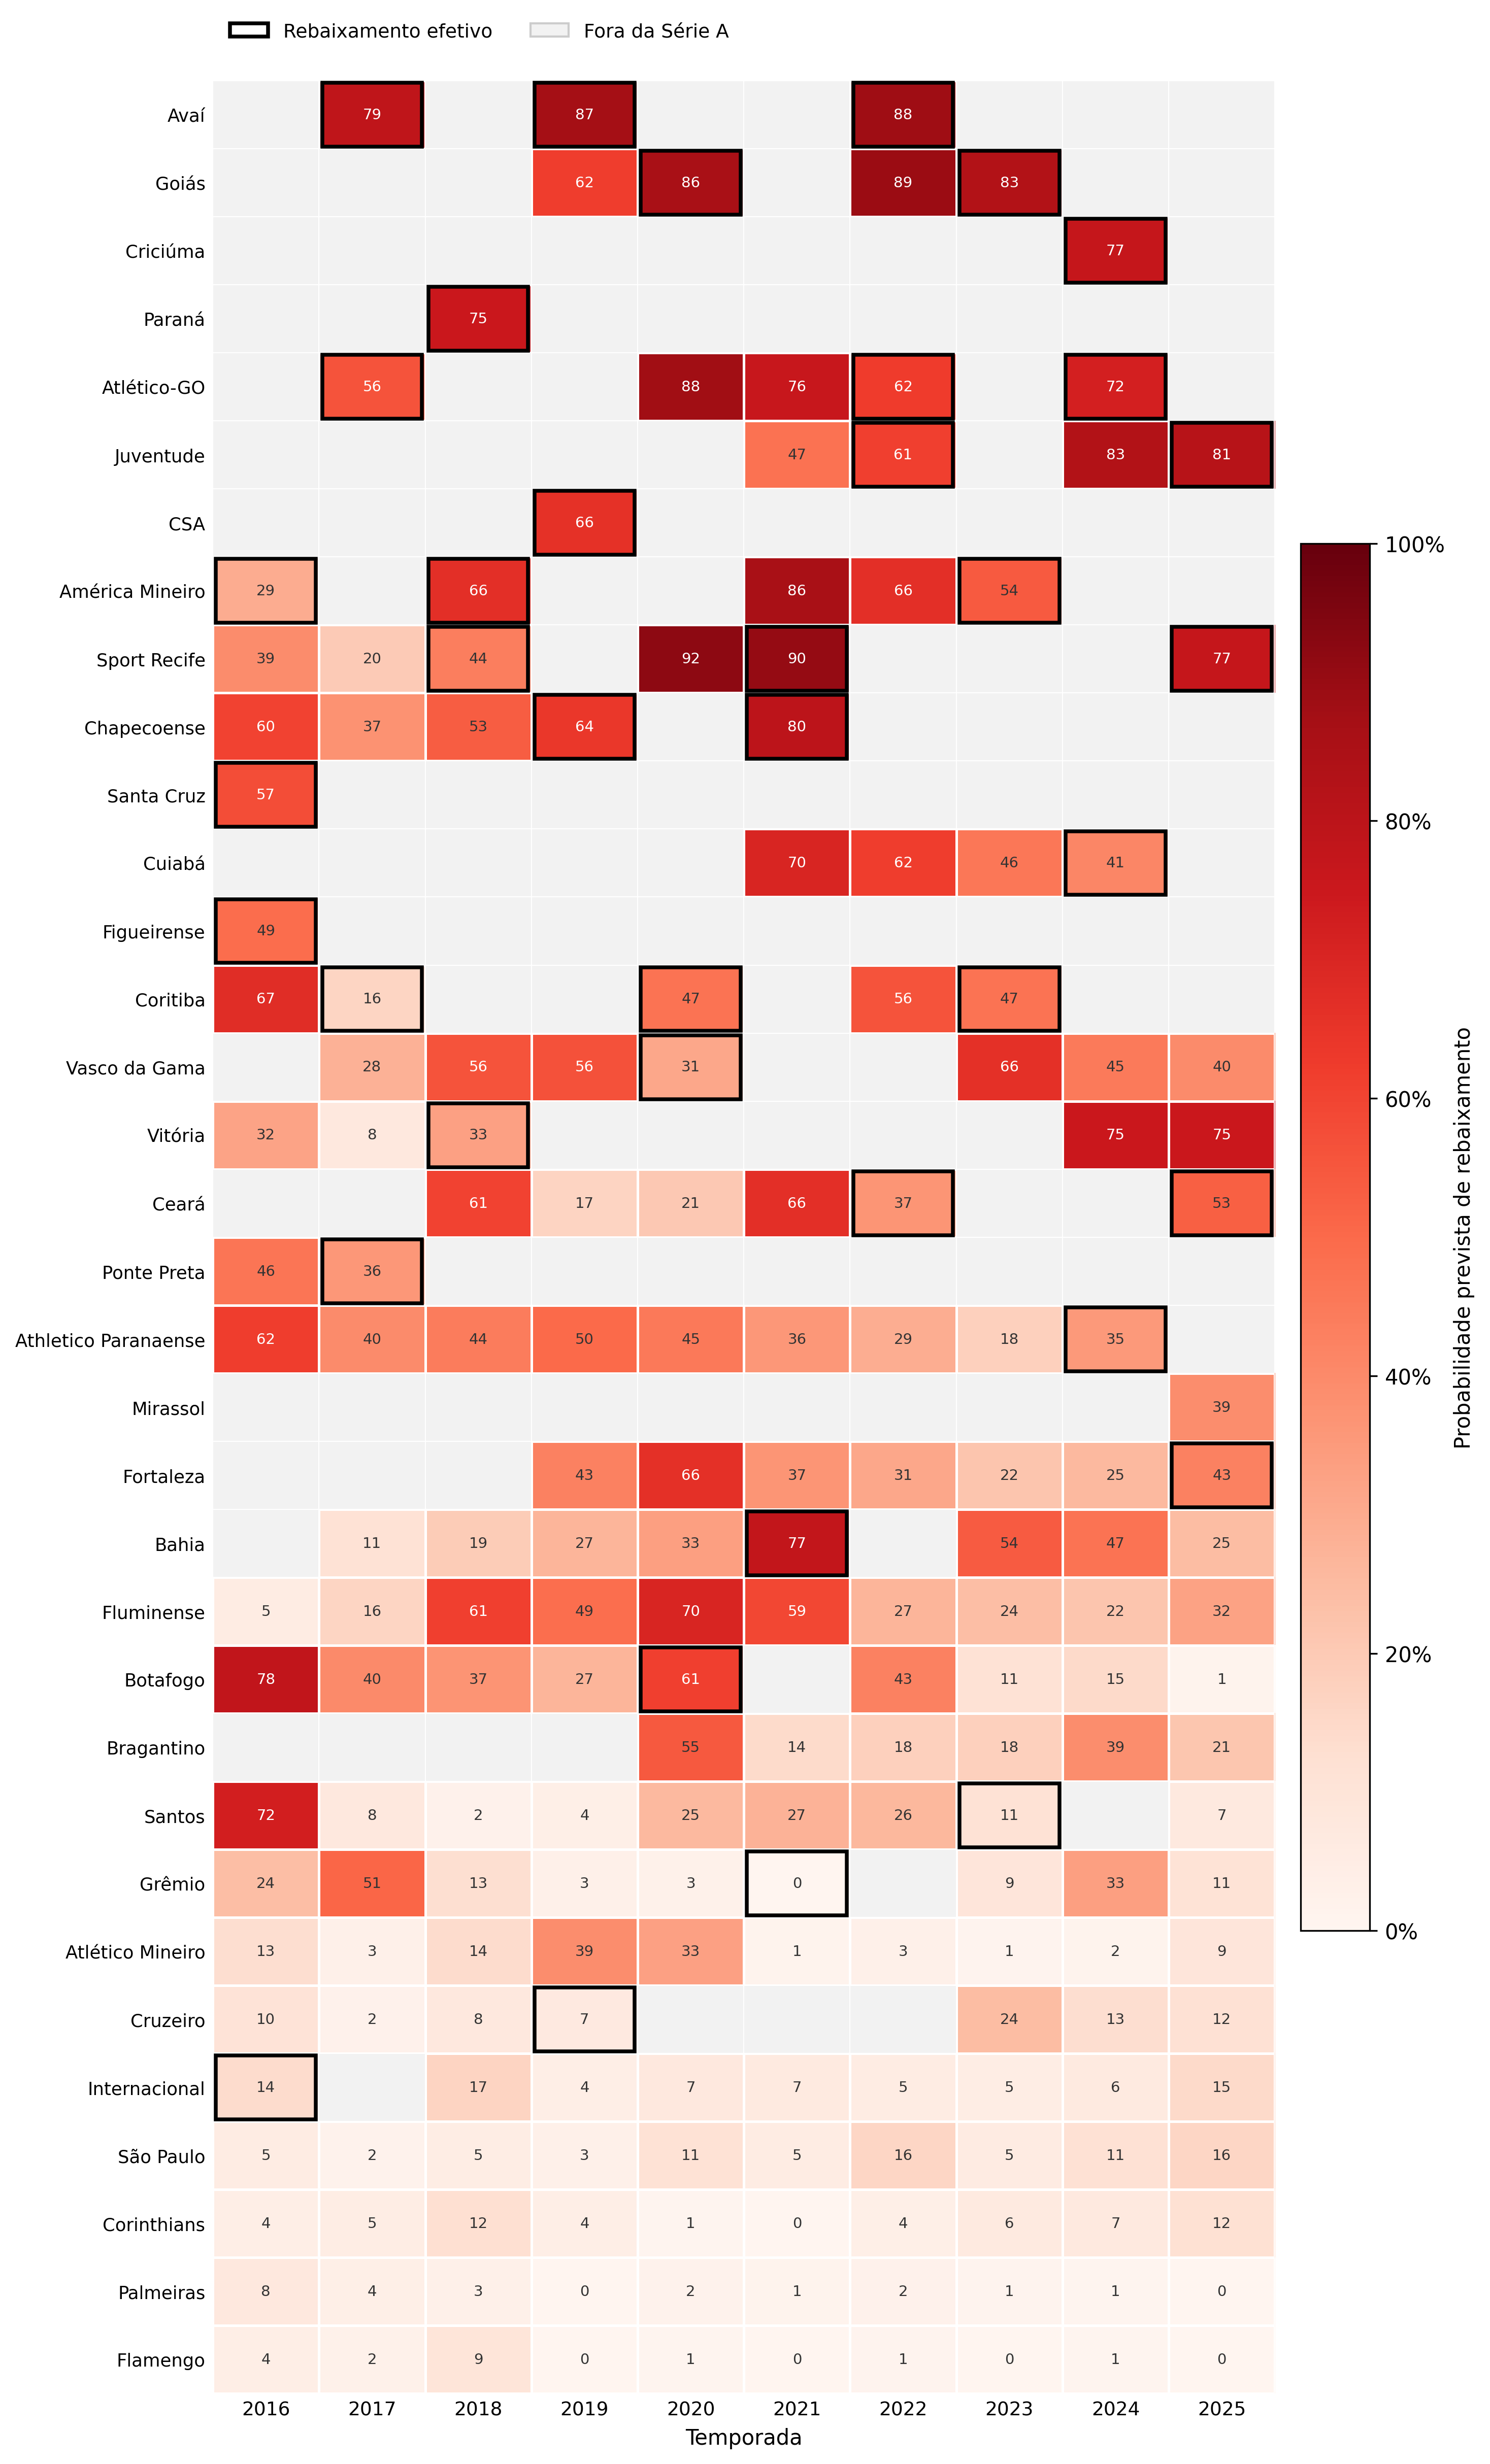
\includegraphics[height=0.72\textheight]{heatmap_risco_longitudinal.png}
    \caption[Mapa de calor longitudinal do risco (2016--2025)]{Mapa de calor longitudinal do risco de rebaixamento (2016--2025): probabilidades previstas pela Regressão Logística retreinada em janela expansiva (apenas temporadas anteriores à prevista). Células contornadas em preto indicam rebaixamentos efetivos; células cinza indicam temporadas fora da Série A. Por adotar protocolo uniforme de retreinamento, os valores de 2025 podem diferir marginalmente dos da Tabela~\ref{tab:previsao2025}.}
    \label{fig:heatmaprisco}

    \small \textit{Fonte: Elaborado pelo autor (\the\year).}
\end{figure}

% ============================================================
% 5. CONSIDERAÇÕES FINAIS
% ============================================================
\section{Considerações Finais}

Este trabalho desenvolveu e comparou quatro modelos de \textit{Machine Learning} para previsão de rebaixamento no Campeonato Brasileiro Série A a partir de informações disponíveis antes do início da temporada. Retomando os objetivos específicos: a base histórica 2014--2025 foi construída com dados do Transfermarkt (objetivo i); a engenharia de \textit{features} com janelas deslizantes foi implementada sem vazamento temporal (objetivo ii); os quatro algoritmos foram treinados e otimizados com validação \textit{walk-forward} e \textit{RandomizedSearchCV} (objetivo iii); a comparação em teste independente apontou o LightGBM como melhor discriminador (AUC-ROC de 0,877, significativamente acima do 0,500 esperado de um classificador aleatório) e a Regressão Logística como modelo mais estável e interpretável (objetivo iv); e a previsão para 2025 foi gerada, indicando Juventude, Sport Recife, Vitória e Mirassol como os clubes de maior risco (objetivo v). A previsão foi, posteriormente, confrontada com os resultados oficiais do campeonato: dois dos quatro rebaixamentos foram antecipados corretamente, os quatro rebaixados reais figuravam entre os sete maiores riscos do ranking e o AUC-ROC realizado na temporada foi de 0,922 --- o melhor entre todos os períodos avaliados, superando ainda heurísticas ingênuas de referência. O objetivo geral foi, portanto, plenamente alcançado.

As contribuições do trabalho são quatro. Primeira, um \textit{pipeline} metodologicamente rigoroso e integralmente reprodutível para previsão esportiva com dados temporais no contexto brasileiro, disponível em repositório público. Segunda, a demonstração empírica da ``armadilha da acurácia'': o contraste entre a acurácia de 82,5\% e o AUC-ROC de 0,652 do XGBoost oferece um exemplo didático da inadequação da acurácia como métrica única em classes desbalanceadas. Terceira, a evidência de que o histórico recente de desempenho, capturado pelas janelas deslizantes, complementa de forma relevante os indicadores financeiros de elenco na explicação do risco de rebaixamento. Quarta, de natureza tecnológica, a entrega do modelo final como uma aplicação web de acesso aberto, que converte o resultado analítico em ferramenta consultável por gestores e pesquisadores, sem exigir a execução do código. A validação retroativa da previsão 2025, com AUC-ROC de 0,922 e superação das heurísticas de referência, converte a previsão apresentada de promessa em resultado verificável --- e os próprios erros do modelo, em especial o caso do Mirassol, delimitam com precisão o alcance da abordagem pré-temporada.

O estudo possui limitações que devem ser reconhecidas. A restrição a dados pré-temporada, embora confira valor prático à previsão, impede que o modelo capture a dinâmica da própria temporada em curso. Fatores sabidamente relevantes --- lesões, trocas de treinador, sobrecarga de calendário e movimentações nas janelas de transferências --- não são modelados. O volume de dados ($\sim$220 observações) é reduzido para os padrões de \textit{Machine Learning}, o que amplia a variância das estimativas, como evidenciado pela oscilação do LightGBM entre \textit{folds} ($\pm$0,151), e limita a complexidade dos modelos treináveis. Por fim, clubes recém-promovidos, sem histórico na Série A, dependem da imputação por mediana, aproximação razoável porém imperfeita de sua realidade competitiva --- o caso do Mirassol em 2025, previsto na zona de rebaixamento e concluindo o campeonato em 4.\textordmasculine{} lugar, é a ilustração mais eloquente dessa limitação. Cabe registrar, por outro lado, que análises de sensibilidade indicaram robustez das principais decisões de projeto: substituir a imputação por mediana pela média não alterou o AUC-ROC no conjunto de teste (0,828 em ambas as configurações), e o uso de janelas de 2 e 4 temporadas produziu resultado equivalente (0,836) ao das janelas de 3 e 5 adotadas.

Como trabalhos futuros, propõe-se: (i) o retreinamento parcial do modelo ao longo da temporada, incorporando a pontuação acumulada para capturar a forma corrente dos clubes; (ii) a inclusão de \textit{features} do mercado de transferências, dado que reforços e vendas impactam diretamente o desempenho esperado; (iii) a experimentação com modelos sequenciais (LSTM, \textit{Transformers}) à medida que mais temporadas ampliem a base de dados; e (iv) a expansão do escopo para a Série B e para ligas de outros países, aumentando o volume de dados e a testabilidade externa das conclusões.

% ============================================================
% REFERÊNCIAS
% ============================================================
\bibliographystyle{abntex2-alf}
\bibliography{referencias}

\end{document}
